\documentclass[10pt,                    % corpo del font principale
               a4paper,                 % carta A4
               twoside,                 % impagina per fronte-retro
               openright,               % inizio capitoli a destra
               english,                 
               italian,                 
               ]{book}    

\usepackage[utf8]{inputenc}           
                                       

%**************************************************************
% Importazione package
%************************************************************** 

\usepackage{amsmath,amssymb,amsthm}    % matematica

\usepackage[english, italian]{babel}    % per scrivere in italiano e in inglese;
									    % l'ultima lingua (l'italiano) risulta predefinita
\usepackage[T1]{fontenc}
     
\usepackage{lmodern} 
                 
\usepackage{bookmark}                   % segnalibri

\usepackage{caption}                    % didascalie

\usepackage{chngpage,calc}              % centra il frontespizio

\usepackage{csquotes}                   % gestisce automaticamente i caratteri (")

\usepackage{emptypage}                  % pagine vuote senza testatina e piede di pagina

\usepackage{epigraph}					% per epigrafi

\usepackage{eurosym}                    % simbolo dell'euro

\usepackage[T1]{fontenc}                % codifica dei font:
                                       
\usepackage{indentfirst}               % rientra il primo paragrafo di ogni sezione

\usepackage{graphicx}                   % immagini

\usepackage{hyperref}                   % collegamenti ipertestuali



\usepackage[binding=5mm]{layaureo}      % margini ottimizzati per l'A4; rilegatura di 5 mm

\usepackage{listings}                   % codici

\usepackage{microtype}                  % microtipografia

\usepackage{mparhack,fixltx2e,relsize}  % finezze tipografiche

\usepackage{nameref}                    % visualizza nome dei riferimenti                                      

\usepackage[font=small]{quoting}        % citazioni

\usepackage{subfig}                     % sottofigure, sottotabelle

\usepackage[italian]{varioref}          % riferimenti completi della pagina

\usepackage[dvipsnames]{xcolor}         % colori

\usepackage{booktabs}                   % tabelle                                       
\usepackage{tabularx}                   % tabelle di larghezza prefissata                                    
\usepackage{longtable}                  % tabelle su più pagine                                        
\usepackage{ltxtable}                   % tabelle su più pagine e adattabili in larghezza

\usepackage[toc, acronym]{glossaries}   % glossario
                                        % per includerlo nel documento bisogna:
                                        % 1. compilare una prima volta tesi.tex;
                                        % 2. eseguire: makeindex -s tesi.ist -t tesi.glg -o tesi.gls tesi.glo
                                        % 3. eseguire: makeindex -s tesi.ist -t tesi.alg -o tesi.acr tesi.acn
                                        % 4. compilare due volte tesi.tex.

\usepackage[backend=biber,style=verbose-ibid,hyperref,backref]{biblatex}
                                        % eccellente pacchetto per la bibliografia; 
                                        % produce uno stile di citazione autore-anno; 
                                        % lo stile "numeric-comp" produce riferimenti numerici
                                        % per includerlo nel documento bisogna:
                                        % 1. compilare una prima volta tesi.tex;
                                        % 2. eseguire: biber tesi
                                        % 3. compilare ancora tesi.tex.

%**************************************************************
% file contenente le impostazioni della tesi
%**************************************************************

%**************************************************************
% Frontespizio
%**************************************************************
\newcommand{\myName}{Simone Magagna}                           % autore
\newcommand{\myTitle}{Realtà virtuale per colmare il divario tra e-commerce e negozio fisico}                    
\newcommand{\myDegree}{Tesi di laurea triennale}                % tipo di tesi
\newcommand{\myUni}{Università degli Studi di Padova}           % università
\newcommand{\myFaculty}{Corso di Laurea in Informatica}         % facoltà
\newcommand{\myDepartment}{Dipartimento di Matematica}          % dipartimento
\newcommand{\myProf}{Tullio Vardanega}                          % relatore
\newcommand{\myLocation}{Padova}                                % dove
\newcommand{\myAA}{2015-2016}                                   % anno accademico
\newcommand{\myTime}{Ottobre 2016}                            % quando
\renewcommand{\lstlistingname}{Code}
\newcommand{\facciatabianca}{\newpage\shipout\null\stepcounter{page}}
%**************************************************************
% Impostazioni di impaginazione
% see: http://wwwcdf.pd.infn.it/AppuntiLinux/a2547.htm
%**************************************************************

\setlength{\parindent}{14pt}   % larghezza rientro della prima riga
\setlength{\parskip}{0pt}   % distanza tra i paragrafi


%**************************************************************
% Impostazioni di biblatex
%**************************************************************
\bibliography{bibliografia} % database di biblatex 

\defbibheading{bibliography}
{
    \cleardoublepage
    \phantomsection 
    \addcontentsline{toc}{chapter}{\bibname}
    \chapter*{\bibname\markboth{\bibname}{\bibname}}
}

\setlength\bibitemsep{1.5\itemsep} % spazio tra entry

\DeclareBibliographyCategory{opere}
\DeclareBibliographyCategory{web}

\addtocategory{opere}{womak:lean-thinking}
\addtocategory{web}{site:agile-manifesto}

\defbibheading{opere}{\section*{Riferimenti bibliografici}}
\defbibheading{web}{\section*{Siti Web consultati}}


%**************************************************************
% Impostazioni di caption
%**************************************************************
\captionsetup{
    tableposition=top,
    figureposition=bottom,
    font=small,
    format=hang,
    labelfont=bf
}

%**************************************************************
% Impostazioni di glossaries
%**************************************************************
\makeglossaries


%**************************************************************
% Impostazioni di graphicx
%**************************************************************
\graphicspath{{immagini/}} % cartella dove sono riposte le immagini


%**************************************************************
% Impostazioni di hyperref
%**************************************************************
\hypersetup{
    %hyperfootnotes=false,
    %pdfpagelabels,
    %draft,	% = elimina tutti i link (utile per stampe in bianco e nero)
    colorlinks=false,
    linktocpage=true,
    pdfstartpage=1,
    pdfstartview=FitV,
    % decommenta la riga seguente per avere link in nero (per esempio per la stampa in bianco e nero)
    %colorlinks=false, linktocpage=false, pdfborder={0 0 0}, pdfstartpage=1, pdfstartview=FitV,
    breaklinks=true,
    pdfpagemode=UseNone,
    pageanchor=true,
    pdfpagemode=UseOutlines,
    plainpages=false,
    bookmarksnumbered,
    bookmarksopen=true,
    bookmarksopenlevel=1,
    hypertexnames=true,
    pdfhighlight=/O,
    %nesting=true,
    %frenchlinks,
    urlcolor=webbrown,
    linkcolor=RoyalBlue,
    citecolor=webgreen,
    %pagecolor=RoyalBlue,
    %urlcolor=Black, linkcolor=Black, citecolor=Black, %pagecolor=Black,
    pdftitle={\myTitle},
    pdfauthor={\textcopyright\ \myName, \myUni, \myFaculty},
    pdfsubject={},
    pdfkeywords={},
    pdfcreator={pdfLaTeX},
    pdfproducer={LaTeX}
}

%**************************************************************
% Impostazioni di itemize
%**************************************************************
\renewcommand{\labelitemi}{$\ast$}

%\renewcommand{\labelitemi}{$\bullet$}
%\renewcommand{\labelitemii}{$\cdot$}
%\renewcommand{\labelitemiii}{$\diamond$}
%\renewcommand{\labelitemiv}{$\ast$}


%**************************************************************
% Impostazioni di listings
%**************************************************************
\lstset{
    language=[LaTeX]Tex,%C++,
    keywordstyle=\color{RoyalBlue}, %\bfseries,
    basicstyle=\small\ttfamily,
    %identifierstyle=\color{NavyBlue},
    commentstyle=\color{Green}\ttfamily,
    stringstyle=\rmfamily,
    numbers=none, %left,%
    numberstyle=\scriptsize, %\tiny
    stepnumber=5,
    numbersep=8pt,
    showstringspaces=false,
    breaklines=true,
    frameround=ftff,
    frame=single
} 


%**************************************************************
% Impostazioni di xcolor
%**************************************************************
\definecolor{webgreen}{rgb}{0,.5,0}
\definecolor{webbrown}{rgb}{.6,0,0}


%**************************************************************
% Altro
%**************************************************************

\newcommand{\omissis}{[\dots\negthinspace]} % produce [...]

% eccezioni all'algoritmo di sillabazione
\hyphenation
{
    ma-cro-istru-zio-ne
    gi-ral-din
}

\newcommand{\sectionname}{sezione}
\addto\captionsitalian{\renewcommand{\figurename}{figura}
                       \renewcommand{\tablename}{tabella}}

\newcommand{\glsfirstoccur}{\ap{{[g]}}}

\newcommand{\intro}[1]{\emph{\textsf{#1}}}

%**************************************************************
% Environment per ``rischi''
%**************************************************************
\newcounter{riskcounter}                % define a counter
\setcounter{riskcounter}{0}             % set the counter to some initial value

%%%% Parameters
% #1: Title
\newenvironment{risk}[1]{
    \refstepcounter{riskcounter}        % increment counter
    \par \noindent                      % start new paragraph
    \textbf{\arabic{riskcounter}. #1}   % display the title before the 
                                        % content of the environment is displayed 
}{
    \par\medskip
}

\newcommand{\riskname}{Rischio}

\newcommand{\riskdescription}[1]{\textbf{\\Descrizione:} #1.}

\newcommand{\risksolution}[1]{\textbf{\\Soluzione:} #1.}

%**************************************************************
% Environment per ``use case''
%**************************************************************
\newcounter{usecasecounter}             % define a counter
\setcounter{usecasecounter}{0}          % set the counter to some initial value

%%%% Parameters
% #1: ID
% #2: Nome
\newenvironment{usecase}[2]{
    \renewcommand{\theusecasecounter}{\usecasename #1}  % this is where the display of 
                                                        % the counter is overwritten/modified
    \refstepcounter{usecasecounter}             % increment counter
    \vspace{10pt}
    \par \noindent                              % start new paragraph
    {\large \textbf{\usecasename #1: #2}}       % display the title before the 
                                                % content of the environment is displayed 
    \medskip
}{
    \medskip
}

\newcommand{\usecasename}{UC}

\newcommand{\usecaseactors}[1]{\textbf{\\Attori Principali:} #1. \vspace{4pt}}
\newcommand{\usecasepre}[1]{\textbf{\\Precondizioni:} #1. \vspace{4pt}}
\newcommand{\usecasedesc}[1]{\textbf{\\Descrizione:} #1. \vspace{4pt}}
\newcommand{\usecasepost}[1]{\textbf{\\Postcondizioni:} #1. \vspace{4pt}}
\newcommand{\usecasealt}[1]{\textbf{\\Scenario Alternativo:} #1. \vspace{4pt}}

%**************************************************************
% Environment per ``namespace description''
%**************************************************************

\newenvironment{namespacedesc}{
    \vspace{10pt}
    \par \noindent                              % start new paragraph
    \begin{description} 
}{
    \end{description}
    \medskip
}

\newcommand{\classdesc}[2]{\item[\textbf{#1:}] #2}                     % file con le impostazioni personali

\begin{document}
%**************************************************************
% Materiale iniziale
%**************************************************************
\frontmatter
%**************************************************************
% Frontespizio 
%**************************************************************
\begin{titlepage}

\begin{center}

\begin{LARGE}
\textbf{\myUni}\\
\end{LARGE}

\vspace{8pt}

\begin{Large}
\textsc{\myDepartment}\\
\end{Large}

\vspace{8pt}

\begin{large}
\textsc{\myFaculty}\\
\end{large}

\vspace{20pt}
\begin{figure}[htbp]
\begin{center}

\includegraphics[height=6cm]{logo-unipd}
\end{center}
\end{figure}
\vspace{30pt} 

\begin{LARGE}
\begin{center}
\textbf{\myTitle}\\
\end{center}
\end{LARGE}

\vspace{10pt} 

\begin{large}
\textsl{\myDegree}\\
\end{large}

\vspace{30pt} 

\begin{large}
\begin{flushleft}
\textit{Relatore}\\ 
\vspace{5pt} 
Prof. \myProf
\end{flushleft}

\vspace{0pt} 

\begin{flushright}
\textit{Laureando}\\ 
\vspace{5pt} 
\myName\\
1009467

\end{flushright}
\end{large}

\vspace{30pt}

\line(1, 0){338} \\
\begin{normalsize}
\textsc{Anno Accademico \myAA}
\end{normalsize}

\end{center}
\end{titlepage} 
%**************************************************************
% Colophon
%**************************************************************
\clearpage
\phantomsection
\thispagestyle{empty}

\hfill

\vfill

\noindent\myName: \textit{\myTitle,}
\myDegree,
\textcopyright\ \myTime.
%**************************************************************
% Dedica
%**************************************************************
\cleardoublepage
\phantomsection
\thispagestyle{empty}
\pdfbookmark{Dedica}{Dedica}

\vspace*{3cm}

\medskip

\begin{center}
Dedica
\end{center}

%**************************************************************
% Sommario
%**************************************************************
\cleardoublepage
\phantomsection
\pdfbookmark{Sommario}{Sommario}
\begingroup
\let\clearpage\relax
\let\cleardoublepage\relax
\let\cleardoublepage\relax

\chapter*{Sommario}

Questo documento rappresenta la relazione finale di stage tenuta presso l'azienda The White Dog s.r.l. della durata complessiva pari a 308 ore. \\
Il primo capitolo tratta dell'azienda ospitante, dei prodotti e dei servizi che offre all’aziende esterne, in particolare all’azienda DIANA: FASHION ECOMMERCE della quale rappresenta il reparto ricerca e sviluppo. \\
Il secondo capitolo descrive le strategie aziendali riguardanti l’attività di stage, di come il mio progetto si integri in esse, del piano di lavoro propostomi e degli obiettivi aziendali e personali. \\
Il terzo capitolo parla dell'effettivo sviluppo del progetto, descrivendo le fasi di pianificazione e ricerca effettuate con il mio tutor aziendale e il team di sviluppo, per arrivare a trattare dell'analisi dei requisiti, dei principi di progettazione perseguiti, dello sviluppo di alcune delle parti più peculiari e interessanti del progetto e della verifica e validazione. \\
Il quarto ed ultimo capitolo analizza i risultati ottenuti confrontandoli con gli obiettivi prefissati, valuta le conoscenze acquisite e discute quali tra queste debbano essere integrate nel corso di studi. Il capitolo si conclude con alcune considerazioni di carattere personale.

%\vfill
%
%\selectlanguage{english}
%\pdfbookmark{Abstract}{Abstract}
%\chapter*{Abstract}
%
%\selectlanguage{italian}

\endgroup			



%**************************************************************
% Ringraziamenti
%**************************************************************
\cleardoublepage

\phantomsection

\pdfbookmark{Ringraziamenti}{ringraziamenti}

\bigskip

\begingroup

\let\clearpage\relax

\let\cleardoublepage\relax

\let\cleardoublepage\relax

\epigraph{\textit{"If you can dream it, you can do it"}}{\textit{Walt Disney}}

\chapter*{Ringraziamenti}

\textit{Ed ecco che infine mi ritrovo a narrare delle mie ultime gesta, della mia ultima e più grande battaglia per la gloria e la vita eterna. Stolto m'incamminai per il tortuoso sentiero, ignaro dei perigli che m'attendevano. Caddi e mi rialzai, piansi e m'asciugai e molte volte la verace via abbandonai. Ma l'animo rimase forte, testarda era la mente, che non scorgeva altre strade se non quella imminente. Vinsi dunque, vinsi contro l'oscurità che più volte attanagliò il mio cuore, contro la fatica che rese incerto il mio passo, ma non vinsi da solo. Molti furono i miei fratelli d'arme in questa rovinosa campagna, molti mi sostennero donandomi la loro spada e il loro scudo. \\ 
Dunque, prima di decantare delle nobili gesta, ritengo d'obbligo ringraziare, ricordare tutti coloro che, con me, combatterono fino alla fine. \\ \\
Ringrazio John Ronald Reuel Tolkien, Oscar Wilde, George Orwell, Isaac Asimov, Voltaire, Fëdor Michajlovič Dostoevskij, Edgar Allan Poe, Douglas Adams, Howard Phillips Lovecraft, Arthur Ignatius Conan Doyle, Stephen Hawking, George Raymond Richard Martin, Joanne Rowling, Dan Brown, Hugo Pratt, Alan Moore, Grant Morrison, Frank Miller, Neil Gaiman, Go Nagai, Yoshiyuki Okamura, Tsugumi Oba, Tsutomu Nihei, Jiro Taniguchi, Valerio Massimo Manfredi, Italo Calvino e tutti i narratori di sogni che hanno allietato con i loro racconti i miei lunghi viaggi. \\ \\
Ringrazio Horward Shore, Hans Zimmer, i Pink Floyd, Bob Marley, Ludovico Einaudi, Fabrizio De André, Giovanni Allevi e tutti i musici che hanno acquietato il mio cuore durante le lunghe notti passate a pianificar battaglie. \\ \\
Ringrazio Valentino, Francesco, Antonio e tutti i membri dell'armata Diana, miei fedeli alleati in questa ultima grande impresa. \\ \\
Ringrazio il professore Tullio Vardanega, per gli insegnamenti donatimi durante questa mia lunga narrazione. \\ \\
Ringrazio il mio Maestro Nicola, i miei compagni Marco, Lara e Federico e la Scuola delle Nove Armonie Conselve, per avermi insegnato molto sulla via del guerriero, per aver sempre combattuto al mio fianco, per non avermi mai lasciato solo nell'oscurità. \\ \\
Ringrazio l'amore mio, la mia Elisa, per aver continuato ad amarmi sempre dopo ogni caduta, aiutandomi a rialzarmi. \\ \\ 
Ringrazio infine mio Padre e mia Madre, per avermi permesso di vivere questa grande e bellissima avventura che è la vita.}

\endgroup
%**************************************************************
% Indici
%**************************************************************
\cleardoublepage
\pdfbookmark{\contentsname}{tableofcontents}
\setcounter{tocdepth}{2}
\tableofcontents
%\markboth{\contentsname}{\contentsname} 
\clearpage

\begingroup 
    \let\clearpage\relax
    \let\cleardoublepage\relax
    \let\cleardoublepage\relax
    %*******************************************************
    % Elenco delle figure
    %*******************************************************    
    \phantomsection
    \pdfbookmark{\listfigurename}{lof}
    \listoffigures

    \vspace*{8ex}

    %*******************************************************
    % Elenco delle tabelle
    %*******************************************************
    \newpage
    \phantomsection
    \pdfbookmark{\listtablename}{lot}
    \listoftables
        
    \vspace*{8ex}
\endgroup

\cleardoublepage

\cleardoublepage
\facciatabianca
%**************************************************************
% Materiale principale
%**************************************************************
\mainmatter
\newpage
%**************************************************************
\chapter{The White Dog s.r.l.}
\label{cap:thewhitedog}

\section{Chi è The White Dog s.r.l.}

The White Dog s.r.l. è una realtà aziendale nata nel 2008 con sede a Torreglia, in provincia di Padova. Essa è stata fondata dal signor Stefano Mocellini, fondatore e CEO di Diana Corp.\footnote[1]{\url{http://www.dianacorp.com/}} , con la volontà di creare un \textit{team} di lavoro focalizzato sulla ricerca e sviluppo. \\
The White Dog s.r.l. coordina e gestisce società tutte affini al settore \textit{e-commerce}, come Diana Corp. e LiveStory\footnote[2]{\url{http://www.livestory.nyc/}}. L'azienda possiede un reparto di ricerca e sviluppo denominato R\&D, il quale esplora nuove tecnologie da applicare poi alle società figlie nel caso di esito positivo o facendo nascere nuovi progetti separati.

\label{The White Dog s.r.l.}
\begin{figure}[ht]
	\begin{center}
		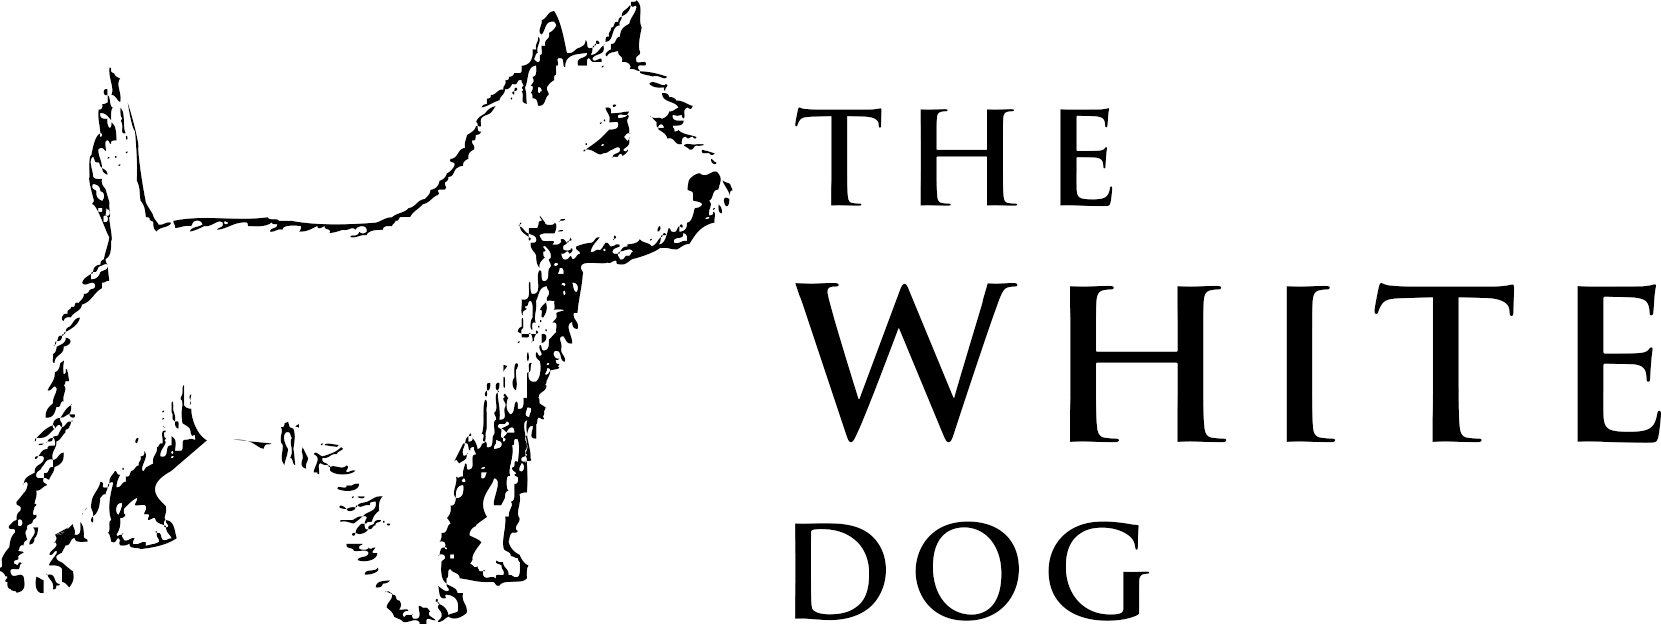
\includegraphics[scale=1]{twd_logo}
		\caption{Logo dell'azienda The White Dog s.r.l.}
	\end{center}
\end{figure}
\FloatBarrier

\section{Prodotti e servizi}

Il principale servizio che l'azienda offre alle aziende che coordina e gestisce, come Diana Corp. e Live Story, è la ricerca e lo sviluppo di nuove tecnologie da applicare nell'ambito del \textit{fashion e-commerce}. Essa svolge l'attività di \textit{testing}\ped{\hyperlink{test}{G}} delle nuove tecnologie web disponibili, le valuta attentamente in termini di prestazioni e costi, per poi renderle disponibili. Ad essa oltretutto vengono commissionati progetti che Diana Corp., per competenze e tempistiche, non può portare a termine, come ad esempio applicazioni \textit{mobile} legate agli \textit{e-commerce} prodotti. \\ \\
The White Dog s.r.l. inoltre ha creato il \textit{concept} di \textit{Live Story}, \textit{social management system}\ped{\hyperlink{sms}{G}} che gestisce contenuti \textit{social} e li rende acquistabili, \textit{concept} che è diventato azienda nel 2015 con sede a New York. \textit{Live Story} colleziona foto degli utenti dei \textit{social network} marcate con un particolare \textit{hashtag} che rappresenta l'azienda che vuole utilizzare il servizio. Il sistema accoppia la foto ad un particolare prodotto presente nel catalogo e genera automaticamente le richieste di permesso di utilizzo della foto e la invia all'utente interessato. Se l'utente approva e il moderatore ritiene conforme la foto, l'azienda può utilizzare il contenuto nel proprio sito o \textit{e-commerce}.

\section{Processi interni}

Lo sviluppo del software a The White Dog s.r.l. segue una metodologia tipicamente Agile\footnote[3]{\url{http://agilemanifesto.org/}}. Questa metodologia permette all'azienda di rispondere in tempi brevi ai continui nuovi bisogni di Diana Corp. e Live Story, anche loro fortemente legate a questo metodo di lavoro. Essendo The White Dog s.r.l. formata da un \textit{team} composto da poche persone, tale metodo di lavoro risulta essere molto efficiente.

\label{Metodologia Agile}
\begin{figure}[ht]
	\begin{center}
		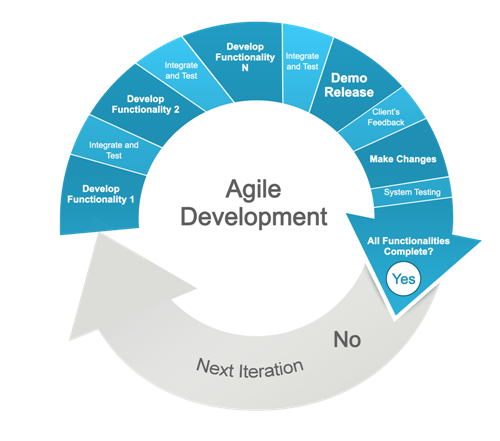
\includegraphics[height=8cm]{agile_development}
		\caption{Metodologia di sviluppo Agile}
	\end{center}
\end{figure}
\FloatBarrier

Le procedure, gli strumenti e le metriche adottate in The White Dog s.r.l. derivano da tre principali concetti di sviluppo Agile:

\subsubsection{DevOps}

Metodologia di sviluppo software che punta alla comunicazione, collaborazione e integrazione tra gli sviluppatori e addetti alle \textit{operations}\ped{\hyperlink{ops}{G}} dell'\textit{information technology}. DevOps vuole rispondere all'interdipendenza tra sviluppo software e IT \textit{operations}\ped{\hyperlink{ops}{G}}, puntando ad aiutare un'organizzazione a sviluppare in modo più rapido ed efficiente prodotti e servizi.

\label{DevOps}
\begin{figure}[ht]
	\begin{center}
		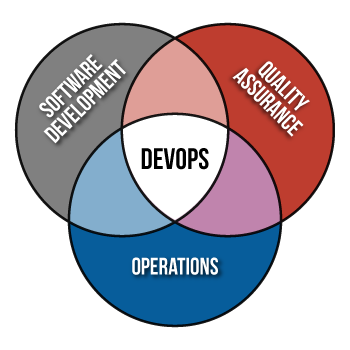
\includegraphics[scale=0.5]{devops-diagram}
		\caption{Competenze necessarie alla metodologia di sviluppo DevOps}
	\end{center}
\end{figure}
\FloatBarrier

In The White Dog s.r.l. questo principio è concretizzato dal fatto che ogni membro possiede sia le competenze di sviluppo, sia amministrative che di controllo della qualità, migliorando così di molto l'efficienza e l'agilità nello sviluppo del software e nel suo rilascio.

\subsubsection{Extreme Programming}

Metodologia di sviluppo software che enfatizza la scrittura di codice di qualità e la rapidità di risposta ai cambiamenti di requisiti. Prescrive lo sviluppo iterativo e incrementale, soprattutto in brevi cicli di sviluppo. Suggerisce inoltre l'uso sistematico di \textit{unit testing}\ped{\hyperlink{ut}{G}} e \textit{refactoring}\ped{\hyperlink{ref}{G}}, vietando ai programmatori di sviluppare codice non strettamente necessario. Sostiene la chiarezza e la semplicità del codice, preferisce strutture gestionali non gerarchiche e dà molta importanza  alla comunicazione diretta e frequente fra sviluppatori e cliente e fra gli sviluppatori stessi. 

\label{Extreme Programming}
\begin{figure}[ht]
	\begin{center}
		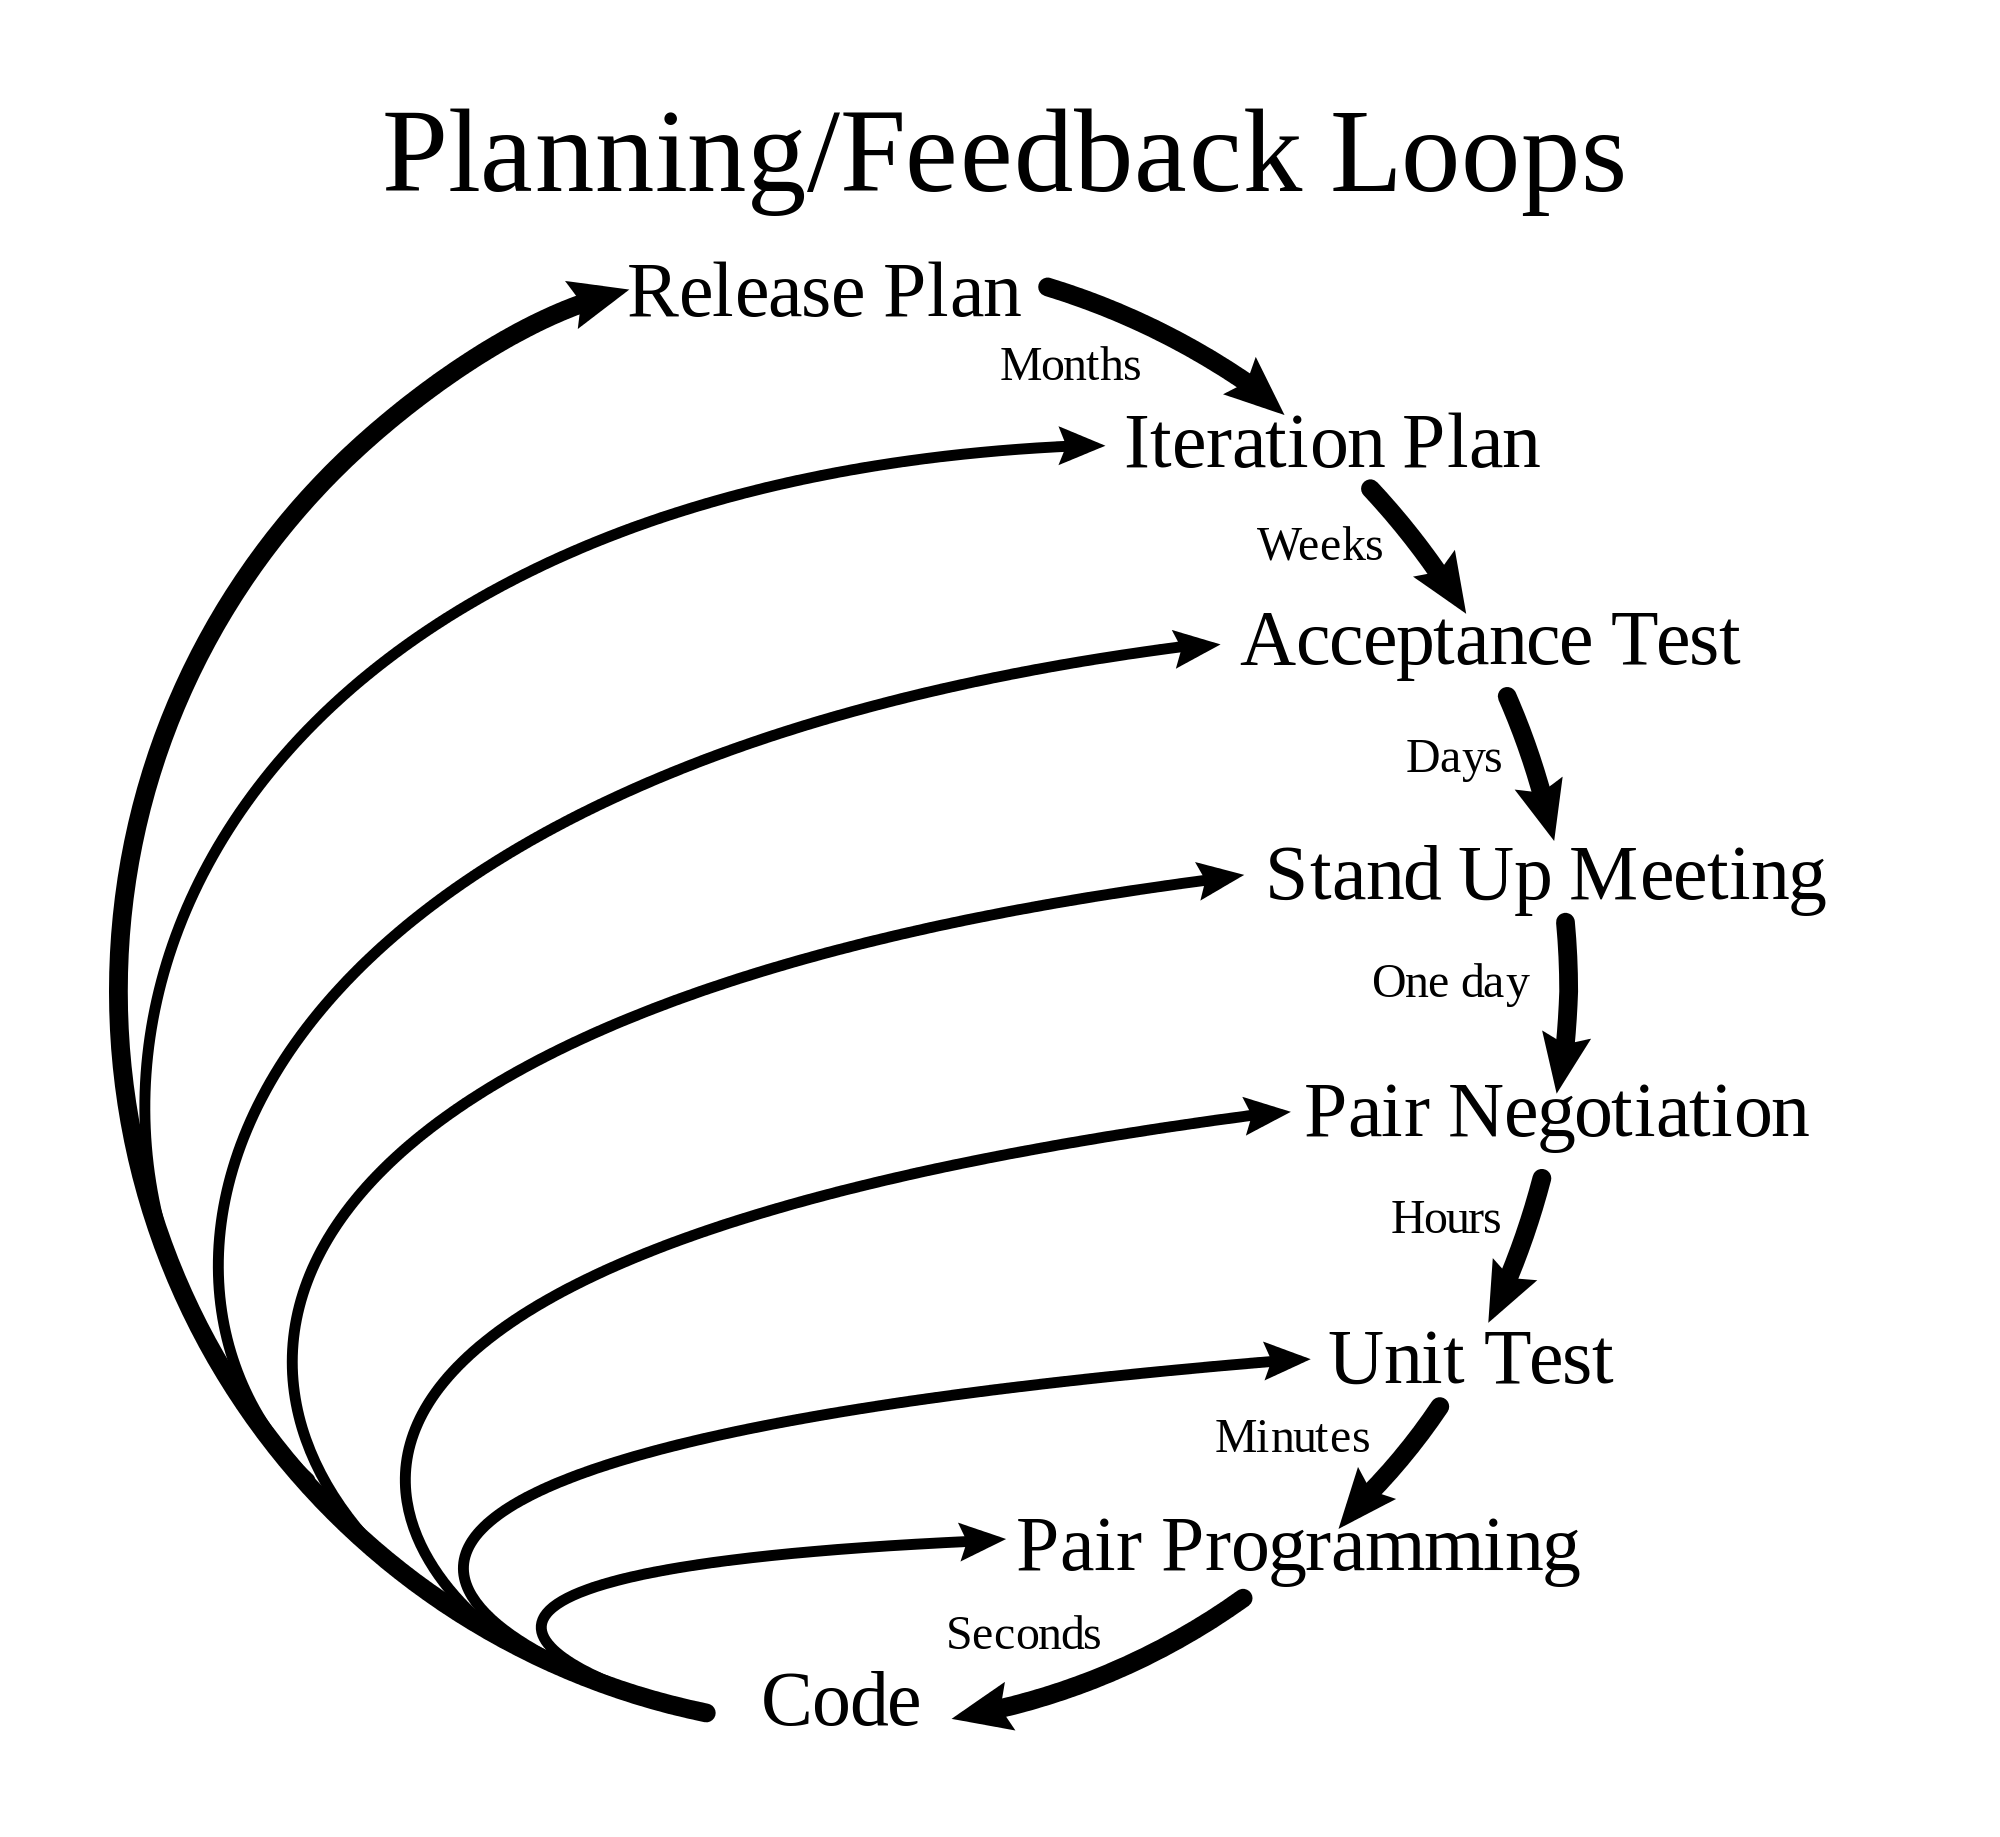
\includegraphics[scale=0.11]{extremeprogramming}
		\caption{Metodologia di sviluppo software Extreme Programming}
	\end{center}
\end{figure}
\FloatBarrier

Il \textit{team} di sviluppo di The White Dog s.r.l. fa ampio utilizzo di questa metodologia, spingendo molto sulla semplicità del codice prodotto, che dovrà poi essere utilizzato dagli sviluppatori Diana Corp. e Live Story, e sulla giornaliera comunicazione diretta tra gli sviluppatori e con i loro principali clienti. Questa comunicazione è facilitata dal fatto che The White Dog s.r.l. ha sede nello stesso stabilimento di Diana Corp..

\subsubsection{Scrum}

\textit{Framework}\ped{\hyperlink{fw}{G}} agile di sviluppo software, iterativo ed incrementale, concepito per gestire progetti e prodotti software. Esso enfatizza tutti gli aspetti di gestione di progetto legati a contesti in cui è difficile pianificare in anticipo. Vengono utilizzati meccanismi propri di un processo di controllo empirico, in cui i cicli di \textit{feedback}, che ne costituiscono le tecniche di \textit{management} fondamentali, risultano in opposizione alla gestione basata sul concetto tradizionale di \textit{command-and-control}\ped{\hyperlink{cac}{G}}. Il suo approccio alla pianificazione e gestione dei progetti è quello di portare l'autorità decisionale al livello di proprietà e certezze operative.

\label{Scrum board}
\begin{figure}[ht]
	\begin{center}
		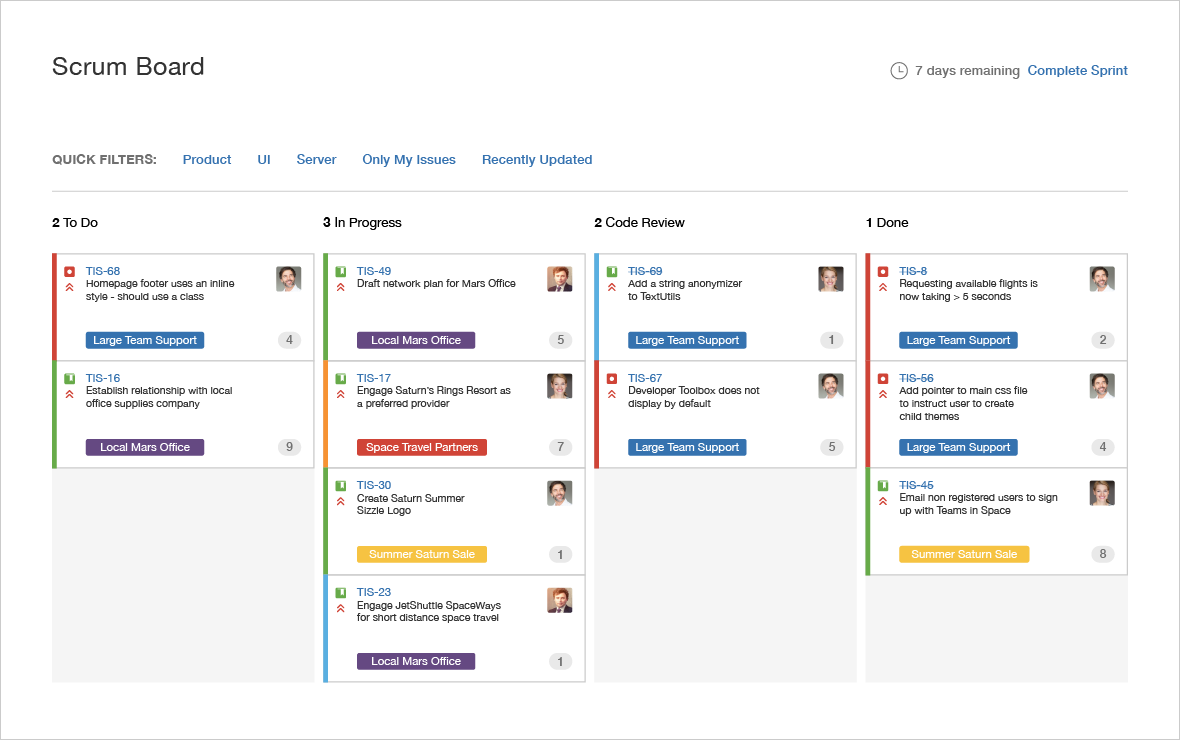
\includegraphics[scale=0.35]{scrumboard}
		\caption{Esempio di \textit{scrum board} all'interno del software Jira}
	\end{center}
\end{figure}
\FloatBarrier

The White Dog s.r.l. sfrutta questa metodologia di sviluppo software utilizzando ampiamente strumenti di \textit{project management} che supportano il metodo Scrum, come Wrike\footnote[4]{\url{https://www.wrike.com/it/it/}} e Jira\footnote[5]{\url{https://www.atlassian.com/software/jira}}.

\section{Strumenti e tecnologie}

\subsection{Ambienti di sviluppo}

Il sistema operativo adottato dall'azienda è Mac OS X installato su macchine iMac. \\
L'ambiente di sviluppo, data la natura aziendale, non è standardizzato, ma varia in base al prodotto in fase di sviluppo, che può cambiare in maniera repentina. 

\subsection{Gestione dei progetti}

I due principali strumenti utilizzati da The White Dog s.r.l. per il \textit{project management} e l'\textit{issue tracking}\ped{\hyperlink{it}{G}} sono rispettivamente Wrike e Jira.\\
Wrike, sviluppato dall'omonima casa, è uno strumento per la collaborazione e il \textit{project management}. Permette ai suoi utenti di modificare progetti, classificare le attività per importanza, tenere traccia dei programmi e collaborare con altri utenti dello stesso gruppo.\\
Jira, prodotto dall'azienda Atlassian, è un software di \textit{bug tracking}\ped{\hyperlink{bg}{G}}, \textit{issue tracking}\ped{\hyperlink{it}{G}} e \textit{project management}. Esso permette di tenere traccia delle azioni e dei problemi degli utenti, di distribuire i compiti all'interno del \textit{team}, discutere del lavoro in atto con una visibilità completa e migliorare le prestazioni della squadra visualizzando dati in tempo reale.

\subsection{Versionamento}

Il principale software di controllo di versione distribuito utilizzato dall'azienda è Git\footnote[6]{\url{https://git-scm.com/}}. Git supporta lo sviluppo non lineare con diramazione e fusioni rapide e continue e comprende strumenti specifici per visualizzare e navigare una cronologia di sviluppo non lineare. Permette ad ogni sviluppatore una copia locale dell'intera cronologia di sviluppo e le modifiche vengono importate da un \textit{repository}\ped{\hyperlink{rep}{G}} ad un altro. I \textit{repository}\ped{\hyperlink{rep}{G}} possono essere pubblicati facilmente tramite protocolli HTTP, FTP, SSH, RSYNC o uno speciale protocollo git.

\subsection{Tecnologie di sviluppo}

Vista la varietà delle ricerche e dei prodotti sviluppati dall'azienda The White Dog s.r.l., le tecnologie di sviluppo sono sempre in continua evoluzione e cambiamento. Le principali sono comunque Java, JavaScript, Node.js, MongoDB, PHP, HTML, CSS e AWS.

\section{Ricerca e innovazione}

R\&D rappresenta il reparto di ricerca e sviluppo dell'azienda The White Dog s.r.l..
Ha a disposizione diversi dispositivi per la ricerca come \textit{smartphone} di ultima generazione, \textit{Smart TV}, \textit{smartwatch} e numerosi dispositivi per lo sviluppo \textit{AR}\ped{\hyperlink{ar}{G}} e \textit{VR}\ped{\hyperlink{vr}{G}} come \textit{Google Glass}, \textit{Oculus Rift Development Kit 2}, \textit{Google Cardboard} e \textit{Leap Motion}. Attraverso questi dispositivi l'azienda studia e sviluppa nuove modalità di interazione che l'utente finale può utilizzare nell'acquisto nei propri \textit{stores} digitali.

\newpage
%**************************************************************
% CAPITOLO 2
%**************************************************************
\chapter{Il quadro strategico}
\label{cap:ilquadrostrategico}

\section{Strategie aziendali di stage}

L'azienda The White Dog s.r.l. accoglie e offre l'attività di stage per due principali motivi:

\begin{itemize}
	\item \textbf{Sperimentazione su progetti innovativi:} data la forte propensione alla ricerca dell'azienda, esistono numerosi campi che essa vorrebbe esplorare ma che a causa di altri progetti più prioritari e scarsità di tempo non può studiare. Offre quindi allo studente universitario un progetto di ricerca e sviluppo su tecnologie innovative ed interessanti, non pretendendo alcun risultato da subito inseribile nel mercato. Questo permette allo studente di vivere l'esperienza dello stage in piena libertà e serenità, riuscendo così a portare un notevole valore aggiunto personale che l'azienda è ben felice di accogliere;
	\item \textbf{Valutazione dello stagista:} l'azienda è in continua crescita e necessita di nuovo personale preparato e soprattutto capace di lavorare in costante sintonia col gruppo. Lo stage universitario permette all'azienda di scoprire persone che soddisfano questi due importanti requisiti per una futura assunzione.
\end{itemize}

Da parte sua The White Dog s.r.l. offre molto agli stagisti. I tutor aziendali supportano lo studente per tutto il periodo lavorativo, consigliandolo sia per quanto riguarda il piano di lavoro, sia sulle tecnologie da utilizzare sia effettuando proficue discussioni in vista della relazione finale. Allo studente viene offerto un ambiente di lavoro accogliente e strumenti aggiornati e all'avanguardia, supportandolo anche economicamente prevedendo un rimborso spese.

\section{Il progetto di stage proposto}

Il progetto propostomi nasce dalla costante volontà aziendale di ricercare nuove metodologie di interazione da proporre agli utenti dei suoi \textit{e-commerce} in ottica \textit{omni-channel}. Il modello \textit{omni-channel} si sta lentamente ma inesorabilmente affermando come principale modello di \textit{retailing}\ped{\hyperlink{ret}{G}} a livello globale e si basa sulle seguenti caratteristiche:

\begin{itemize}
	\item Concezione e management unitario della distribuzione;
	\item Processi basati sull'interazione, comunicazione e interdipendenza tra i \textit{team} dedicati ai singoli canali;
	\item Approccio dinamico al consumatore, che richiede un monitoraggio in tempo reale delle evoluzioni dei comportamenti di acquisto e delle risposte alle iniziative promosse;
	\item Predisposizione di adeguati strumenti IT e marketing in grado di sfruttare ed assecondare il fenomeno della cross-canalità dei processi di acquisto;
	\item Impatto competitivo decisivo delle scelte organizzative e di investimento nell'IT e nel marketing digitale;
	\item Impiego di indicatori di prestazioni e di sistemi di \textit{monitoring} adeguati al nuovo contesto.
\end{itemize}

Questo significa, da parte delle aziende, offrire un'unica \textit{customer experience} capace di rispondere in modo adeguato alle aspettative del consumatore omnicanale che si informa sui prodotti in mobilità, li prova e li sperimenta in negozio per poi acquistarli in loco o online. In termini pratici, questo si implementa costruendo un unico profilo del consumatore, immagazzinandovi dati sulle ricerche da lui effettuate, sulle scelte e sui dati personali immessi per poi sfruttarli in ogni tipologia di \textit{store}, sia digitale che fisico. \\
La realtà virtuale si pone nella strategia \textit{omni-channel} come punto di connessione tra \textit{store} digitale e fisico, permettendo all'utente di esplorare il negozio nella sua totalità e di osservarne i prodotti esposti da più angolazioni o indossati da modelli o manichini, nel caso dei capi di abbigliamento, il tutto con un alto livello di definizione. 
Nasce così l'idea di un \textit{e-commerce VR}, progetto in grado di colmare, in parte, quel divario che da sempre ha distanziato \textit{store} virtuale e negozio fisico.

\label{Omni-channel}
\begin{figure}[ht]
	\begin{center}
		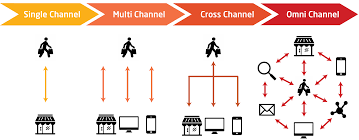
\includegraphics[scale=0.47]{omni-channel}
		\caption{Schema rappresentativo della differenze tra \textit{single-channel}, \textit{multi-channel}, \textit{cross-channel} e \textit{omni-channel}. Immagine tratta dal sito dell'azienda ON THE MARK: \url{http://on-the-mark.com/omnichannel-organization-designs-biggest-test/}}
	\end{center}
\end{figure}
\FloatBarrier

L'obbiettivo di stage è, dunque, un'esplorazione tecnologica nel campo della \textit{virtual reality}\ped{\hyperlink{vr}{G}}. Il progetto mira ad arrivare ad un prototipo di \textit{virtual showroom} dove poter esplorare ed interagire con i prodotti e permetterne l'acquisto. \\
Il progetto era stato inizialmente diviso in due parti, per due differenti studenti:
\begin{itemize}
	\item La prima parte riguardava la progettazione e realizzazione del movimento in uno spazio 3D ed interazione con gli oggetti;
	\item La seconda parte trattava, invece, la progettazione e realizzazione di un'interfaccia di presentazione del prodotto, con integrazione al processo di acquisto mediante l'uso di sistemi \textit{cloud} esterni.
\end{itemize}
Purtroppo, nessun altro studente oltre a me ha aderito al progetto, dunque abbiamo ritenuto opportuno rivisitare l'obbiettivo di stage. Dopo una riunione effettuata prima dell'inizio dello stage con il mio tutor aziendale, abbiamo deciso di mantenere intatti tutti gli obiettivi di ricerca, abbassando il livello qualitativo richiesto. Questo perché lo scopo ultimo di questo stage non era sviluppare un'applicazione o un servizio immediatamente vendibile, ma di studiare le potenzialità e i limiti di questa nuova tecnologia. Questa volontà è stata dettata anche dal fatto che il \textit{team} aziendale inizialmente non aveva alcuna certezza che la tecnologia \textit{VR}\ped{\hyperlink{vr}{G}} fosse applicabile al mondo \textit{e-commerce}.

\subsection{Piano di lavoro proposto}

\subsubsection{Piano temporale}

In accordo col tutor aziendale, la durata massima dello stage è stata fissata a 320 ore, divise in 8 settimane lavorative di 5 giorni, 8 ore al giorno. \\
Il piano lavorativo è stato dunque pianificato per settimana nel seguente modo:

\begin{itemize}
	\item \textbf{Settimana 1:} settimana dedicata completamente alla ricerca, per colmare il \textit{deficit} culturale personale e aziendale sulle tecnologie \textit{VR}\ped{\hyperlink{vr}{G}}. Le attività principali previste sono: analisi dei requisiti funzionali del sistema da sviluppare e studio delle tecnologie e linguaggi disponibili riguardanti la realtà virtuale;
	
	\item \textbf{Settimana 2:} in base ai risultati ottenuti nella prima settimana, viene richiesta una scelta dell'hardware da utilizzare e un \textit{framework}\ped{\hyperlink{fw}{G}} di sviluppo, testandoli con un primo prototipo di scena 3D;
	
	\item \textbf{Settimana 3:} previste attività di raffinamento della scena 3D, progettazione e sviluppo degli oggetti e loro comportamento nello spazio 3D. Viene creato così un primo prototipo di \textit{user interaction};
	
	\item \textbf{Settimana 4:} previste attività di progettazione e sviluppo integrazione tra sistema \textit{VR}\ped{\hyperlink{vr}{G}} e \textit{e-commerce}. Progettazione di \textit{user interaction} per la fruizione dei contenuti provenienti dall'\textit{e-commerce};
	
	\item \textbf{Settimana 5:} settimana dedicata all'approfondimento di \textit{user interaction} e del comportamento degli oggetti nell'ambiente virtuale;
	
	\item \textbf{Settimana 6:} previste attività di studio e prototipazione del possibile processo d'acquisto all'interno dell'ambiente virtuale;
	
	\item \textbf{Settimana 7:} la settima settimana rappresenta una \textit{milestone} importate per il progetto: conclusione del prototipo e relativa documentazione, raggiungendo così gli obbiettivi minimi;
	
	\item \textbf{Settimana 8:} l'ultima settimana viene dedicata completamente allo studio del modello emergente \textit{omni-channel}\ped{\hyperlink{oc}{G}} e come la realtà virtuale possa estendere questo modello. Vengono così raggiunti gli obbiettivi massimi.
\end{itemize}

\subsubsection{Piano metodologico}
	
Assieme al tutor aziendale, abbiamo fin da subito concordato la mia presenza durante l'orario d'ufficio, permettendo così un interazione intensa e costante. \\
Il lavoro di ricerca e sviluppo che ho effettuato è stato totalmente autonomo, con giornaliere interazioni con il personale solo per raccogliere e analizzare la documentazione, requisiti e \textit{feedback} sull'andamento del progetto. \\
Le revisioni di progetto sono avvenute secondo la seguente metodologia:

\begin{itemize}
	\item Riunione breve di 15 minuti ogni mattina;
	\item Riunione di 1 ora alla fine di ogni settimana come analisi retrospettiva.
\end{itemize}

Alle revisioni, oltre a me, hanno partecipato:

\begin{itemize}
	\item \textbf{Valentino Baraldo}, \textit{cloud engineer} e tutor aziendale. Oltre a svolgere il compito di tutor aziendale, mi ha supportato sulla progettazione architetturale del progetto e sull'utilizzo del servizio \textit{API Gateway} di \textit{Amazon Web Services}\footnote[1]{\url{https://aws.amazon.com/it/}};
	\item \textbf{Francesco Paggin}, \textit{front-end developer}. Ha supervisionato il mio lavoro grafico nell'ambiente di sviluppo \textit{Unity}\footnote[2]{\url{https://unity3d.com/}}.
\end{itemize}  

\subsubsection{Piano tecnologico}

Inizialmente lo \textit{stack} tecnologico propostomi riguardava solamente l'hardware che l'azienda aveva acquistato per questo progetto, senza alcun vincolo software. I dispositivi che permettevano la sperimentazione \textit{VR}\ped{\hyperlink{vr}{G}} erano:

\begin{itemize}
	\item \textbf{Oculus Rift Development kit 2:} visore per la realtà virtuale per uso desktop. Possiede uno schermo Samsung OLED 2160x1200 pixel (1080x1200 per occhio), con un \textit{refresh rate} a 90 Hz e un ampio angolo di visione a 110 gradi. Dotato di accelerometro, giroscopio, magnetometro e \textit{tracking} posizionale a 360 gradi. Viene accoppiato ad una telecamera infrarossi per il rilevamento di profondità, assieme a 40 emettitori infrarossi all'interno dell'\textit{headset}. Monta due lenti in alta definizione possedendo 6 gradi di libertà di rotazione;
	
	\item \textbf{Samsung Gear VR:} visore per la realtà virtuale per uso \textit{mobile}. Possiede: accelerometro, giroscopio e sensore di prossimità, permettendo un campo visivo di 96 gradi. Il visore incorpora inoltre un'interfaccia utente fisica: \textit{touch pad}, tasto indietro e tasto per il volume. Necessita l'inserimento di uno \textit{smartphone} Samsung a partire dalla versione \textit{Galaxy S6};
	
	\item \textbf{Google Cardboard:} con il termine \textit{Google Cardboard} non si intende specificare un particolare visore per la realtà virtuale prodotto fisicamente da \textit{Google}, ma un insieme di linee guida suggerite da questa per costruire un dispositivo a basso costo per l'uso \textit{mobile}. In azienda erano presenti due visori che implementavano tali linee guida: \textit{Unofficial Cardboard} e \textit{Tera VR Box};
	
	\item \textbf{Leap Motion:} piccola periferica USB  progettata per essere posta su una scrivania reale rivolta verso l'alto. Usando 2 telecamere e 3 LED infrarossi essa osserva un'area approssimativamente a forma di semisfera di circa un metro. E' progettata per identificare dita o oggetti simili come una penna, con una precisione di 0,01 mm. 
\end{itemize}

\label{Gear VR}
\begin{figure}[ht]
	\begin{center}
		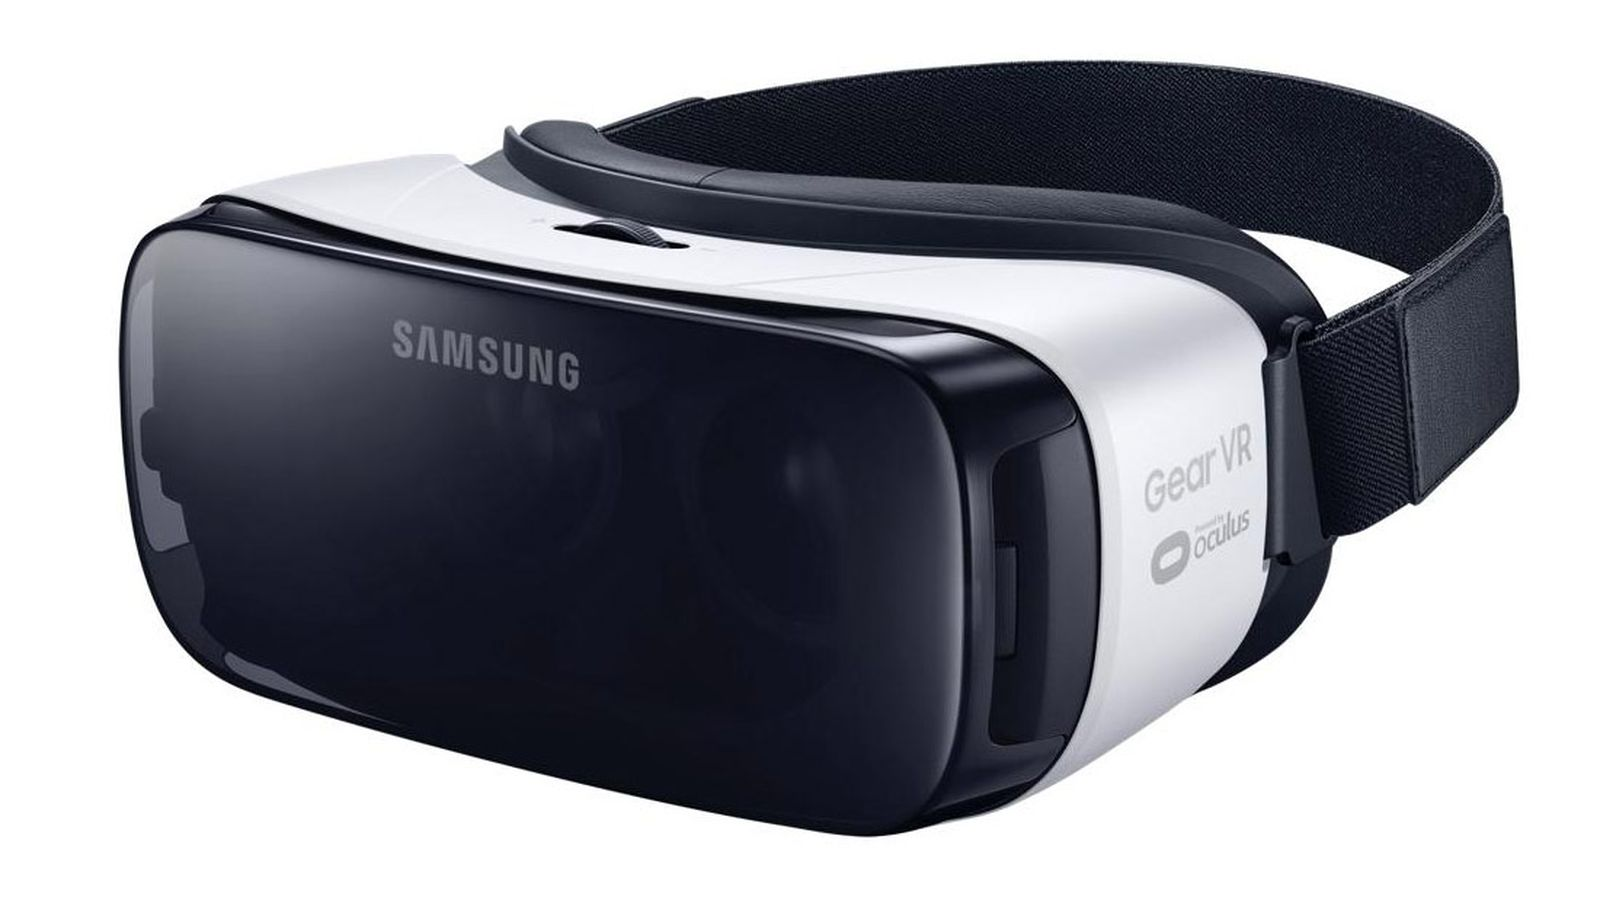
\includegraphics[scale=0.15]{gearvr}
		\caption{Samsung Gear VR}
	\end{center}
\end{figure}
\FloatBarrier

Dopo un periodo di ricerca e \textit{testing} su queste tecnologie, abbiamo deciso di intraprendere la strada \textit{mobile} a discapito di quella desktop. Questa decisione è stata dettata principalmente da due fattori:

\begin{itemize}
	\item \textbf{Requisiti hardware elevati}: per poter offrire un esperienza fluida e piacevole, \textit{Oculus Rift Development kit 2} abbisogna di un PC dall'hardware elevato, non accessibile all'utenza media:
	\begin{itemize}
		\item \textbf{GPU:} NVIDIA GTX 970 / AMD R9 290;
		\item \textbf{CPU:} Intel i5-4590;
		\item \textbf{RAM:} 8GB;
		\item \textbf{Video output:} HDMI 1.3;
		\item \textbf{USB Ports:} 3 porte 3.0 più una porta 2.0;
		\item \textbf{OS:} Windows 7 SP1 64 bit o superiore.
	\end{itemize}
	
	\item \textbf{Obiettivi aziendali:} nonostante fin da subito mi sia stato chiarito che non veniva preteso alcun prodotto finale utilizzabile, l'azienda sperava però di riuscire, con questo stage, a sviluppare un primo prototipo di \textit{virtual showroom} da poter mostrare alle fiere tecnologiche alle quali partecipa. In quest'ottica, l'utilizzo di \textit{Oculus Rift Development kit 2} sarebbe risultato troppo scomodo sia per il trasporto e l'installazione, che per l'utilizzatore finale.
\end{itemize}

Abbiamo deciso, dunque, di sviluppare sia per \textit{Samsung Gear VR} che per \textit{Google Cardboard}, entrambi dispositivi \textit{mobile} a costo contenuto. \\
Lo stack software che si è andato a formare poi, presa questa decisione, ha avuto un tempo decisionale assai breve. Dopo alcune ricerche da me effettuate, ho potuto riscontrare come \textit{Unity} fosse l'unico \textit{framework}\ped{\hyperlink{fw}{G}} per lo sviluppo \textit{VR}\ped{\hyperlink{vr}{G}} gratuito e ricco di documentazione, cosa estremamente fondamentale data la mia iniziale totale ignoranza sull'argomento. \\
\textit{Unity} è uno strumento di \textit{authoring}\ped{\hyperlink{auth}{G}} integrato e multipiattaforma per la creazione di videogiochi 3D o altri contenuti interattivi, quali visualizzazioni architettoniche o animazioni 3D in tempo reale. Esso, tramite gli \textit{SDK}\ped{\hyperlink{sdk}{G}} forniti da Samsung, per il dispositivo Gear VR, da Google, per il dispositivo Cardboard, e da Andriod, per l'interfacciamento con lo smartphone, permette lo sviluppo di applicazioni \textit{VR}\ped{\hyperlink{vr}{G}} fornendo un interfaccia per modellare "a mano" gli oggetti presenti nella scena e i linguaggi JavaScript e C\# per svilupparne il comportamento. \\
Il linguaggio di \textit{scripting} da me scelto per modellare il comportamento degli oggetti nello spazio tridimensionale è C\#, poiché è risultato essere il linguaggio più utilizzato nella \textit{community} \textit{Unity}.

\label{Stack Gear VR}
\begin{figure}[ht]
	\begin{center}
		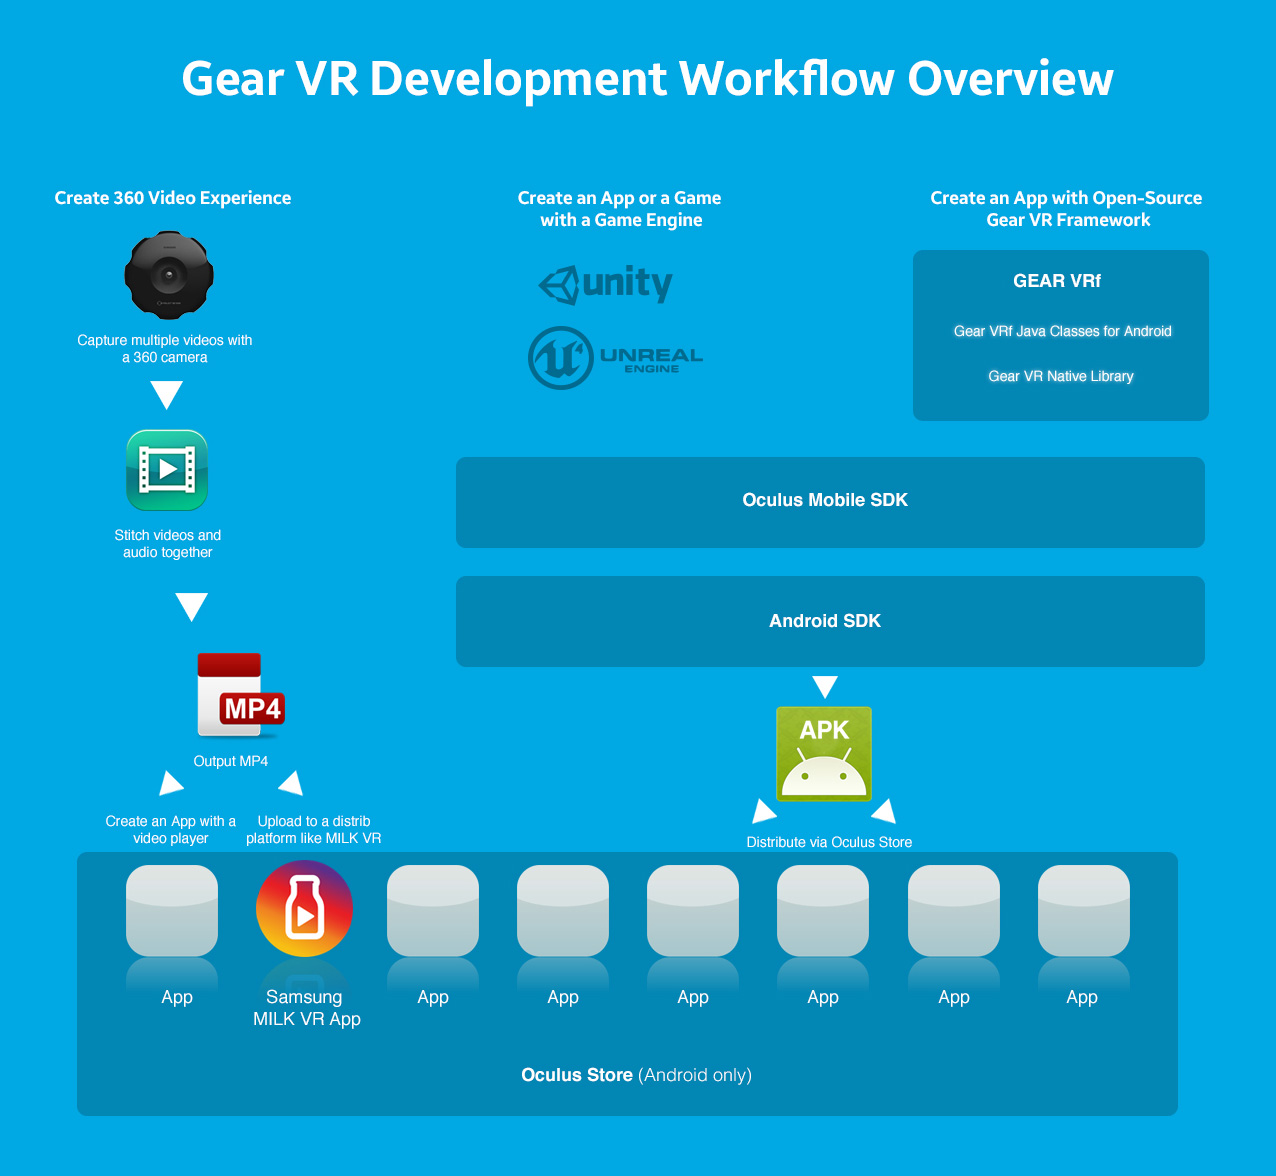
\includegraphics[scale=0.28]{stack-gearvr}
		\caption{Stack tecnologico di sviluppo per Samsung Gear VR. Immagine tratta dal sito SAMSUNG GEAR VR DEVELOPERS US: \url{http://www.samsung.com/us/samsungdeveloperconnection/developer-resources/gear-vr.html}}
	\end{center}
\end{figure}
\FloatBarrier

\subsection{Obiettivi aziendali}

Nel \textit{Piano di Lavoro} presentatomi, l'azienda espone gli obbiettivi minimi e massimi che si aspetta di veder raggiunti alla fine delle 320 ore si stage:

\begin{itemize}
	\item \textbf{Obbiettivi minimi:}
	\begin{enumerate}
		\item Studio delle tecnologie disponibili in ambito \textit{VR}\ped{\hyperlink{vr}{G}} e stesura di un documento riassuntivo che offra un \textit{overview} dello stato attuale della realtà aumentata;
		\item Progettazione e sviluppo di un ambiente virtuale con: una scena e oggetti definiti, un comportamento associato agli oggetti, un prototipo di \textit{user interaction} e scambio di informazioni di base con un sistema di \textit{e-commerce}.
	\end{enumerate}
	\item \textbf{Obbiettivi massimi:}
	\begin{enumerate}
		\item Studio e prototipazione di diversi modelli di \textit{user interaction} con l'ambiente e con gli oggetti finalizzati alla presentazione di un bene vendibile;
		\item Studio e implementazione di possibili nuovi processi di acquisto in ambito \textit{VR}\ped{\hyperlink{vr}{G}}. 
	\end{enumerate}
\end{itemize}

\subsection{Obiettivi personali}

Sono venuto a conoscenza di questo progetto durante l'evento di Stage IT 2016, organizzato da Confindustria Padova in collaborazione con l'Università di Padova e Venezia. Mi ha fin da subito colpito e appassionato per le tecnologie che mi avrebbe permesso di studiare, come ad esempio \textit{Unity}. La computer grafica è da sempre un mio personale interesse e la realtà aumentata è un ambito per me molto affascinante e ricco di opportunità. \\
Le tecnologie proposte dall'azienda purtroppo non rientrano nel percorso di studi, dunque gli obbiettivi formativi personali che mi sono posto riguardano lo studio e la sperimentazione delle tecnologie, senza pretendere di arrivare ad un risultato non prototipale:

\begin{itemize}
	\item \textbf{Obiettivi minimi:}
	\begin{enumerate}
		\item Conoscenza ad alto livello delle tecnologie (hardware e software) attualmente disponibili nel mercato atte a creare ambienti virtuali;
		\item Conoscenza ad alto livello dei concetti principali di \textit{e-commerce} e relative tecnologie di riferimento usate per la vendita online.
	\end{enumerate}
	\item \textbf{Obiettivi massimi:}
	\begin{enumerate}
		\item Capacità di identificare, progettare e sviluppare ambienti virtuali, selezionando le tecnologie attualmente disponibili più appropriate per il caso d'uso;
		\item Presa di coscienza dei concetti multi-channel e omni-channel e come le nuove modalità di vendita si integrino con questi modelli emergenti.
	\end{enumerate}
\end{itemize}            
\newpage
%**************************************************************
% CAPITOLO 3
%**************************************************************

\chapter{Il progetto di e-commerce VR}
\label{cap:ilprogettoe-commercevr}

\section{Analisi dei requisiti}

Questa sezione tratta dei casi d'uso e dei requisiti che il \textit{team} ha ricavato durante la discussione nella prima riunione di stage. Tale analisi ha subito un sostanzioso cambiamento durante la settimana 6, settimana dedicata alla prototipazione del possibile processo d'acquisto all'interno dell'ambiente virtuale. A causa della sua scarsa usabilità, abbiamo deciso di non utilizzare una tastiera virtuale all'interno dell'ambiente tridimensionale per dare la possibilità all'utente di immettere i propri dati e gli estremi di pagamento. Ciò ha portato il \textit{team} a prevedere una registrazione ad un normale sito di \textit{e-commerce} prima di effettuare l'autenticazione all'app, dove dar la possibilità all'utente di immettere i propri dati di pagamento. La sezione 3.2.2 spiega in maniera approfondita le sperimentazioni e le discussioni effettuate che hanno portato a questa importante decisione. 


\subsection{Caratteristiche degli utenti}

Obbligare l'utente ad immettere dati sensibili e strettamente personali, come gli estremi di pagamento, prima dell'effettivo utilizzo del servizio non è una buona prassi. L'utente, che si appresta per la prima volta ad utilizzare l'applicazione, potrebbe non conoscere l'azienda di produzione e potrebbe non fidarsi. Dunque sono stati delineati due principali tipologie d'utente:

\begin{itemize}
	\item \textbf{Utente registrato visitatore:} utente che ha effettuato la registrazione ma che ha deciso di non immettere i propri dati della carta di credito. Ad esso è permesso visualizzare l'ambiente \textit{VR}\ped{\hyperlink{vr}{G}}, selezionare i prodotti e conoscerne le caratteristiche, aggiungerli al carrello, che sarà reso persistente, ma non di concluderne l'acquisto;
	\item \textbf{Utente registrato acquirente:} utente che ha effettuato la registrazione immettendo anche i dati della carta di credito. Ad esso è permessa la totale esperienza incluso l'acquisto dei prodotti presenti nel carrello.
\end{itemize}

\label{Gerarchia utenti}
\begin{figure}[ht]
	\begin{center}
		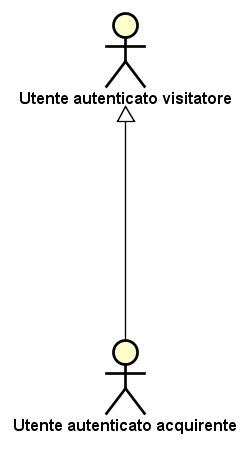
\includegraphics[scale=0.8]{utenti}
		\caption{Gerarchia degli utenti. L'utente autenticato acquirente può effettuare tutte le operazioni dell'utente registrato visitatore ma in più ha la possibilità di acquistare gli oggetti presenti nel carrello}
	\end{center}
\end{figure}
\FloatBarrier

\subsection{Casi d'uso}

Verranno di seguito elencati tutti i casi d'uso individuati dal \textit{team} per l'applicazione, che spiegano in che modo un utente possa interagire con l'applicazione. Per ogni caso d'uso viene mostrato uno schema \textit{UML}\hyperlink{uml}{G} che ne rappresenta il flusso operativo. \\ 
Non vengono considerati i casi d'uso relativi alla registrazione al sito/e-commerce poiché tale funzionalità non è stata da me implementata non essendo di mia competenza.

\subsubsection{Caso d'uso UC1: Autenticazione}

\begin{itemize}
	\item \textbf{Attori:} utente registrato visitatore, utente registrato acquirente;
	\item \textbf{Descrizione:} prima dell'ambiente virtuale, l'utente viene invitato ad immettere l'\textit{username} e la \textit{passowrd} scelti in fase di registrazione all'interno di una scena 2D. Potrà immettere tali dati manualmente utilizzando la normale tastiera del proprio telefono;
	\item \textbf{Precondizione:} l'applicazione è avviata e mostra la pagina di login;
	\item \textbf{Postcondizione:} l'autenticazione è andata a buon fine e l'applicazione passa in modalità \textit{VR}\ped{\hyperlink{vr}{G}}.
	\item \textbf{Scenario principale:}
	\begin{enumerate}
		\item L'utente può inserire l'\textit{username} (UC1.1);
		\item L'utente può inserire la \textit{passowrd} (UC1.2);
		\item L'utente può confermare i dati inseriti premendo sul pulsante di login (UC1.3).
	\end{enumerate}
	\item \textbf{Estensioni:} L'utente può visualizzare un messaggio di errore se i dati immessi non corrispondono a quelli di registrazione o se il campo \textit{username} e \textit{passowrd} sono vuoti (UC1.4).
\end{itemize}

\label{UC1}
\begin{figure}[ht]
	\begin{center}
		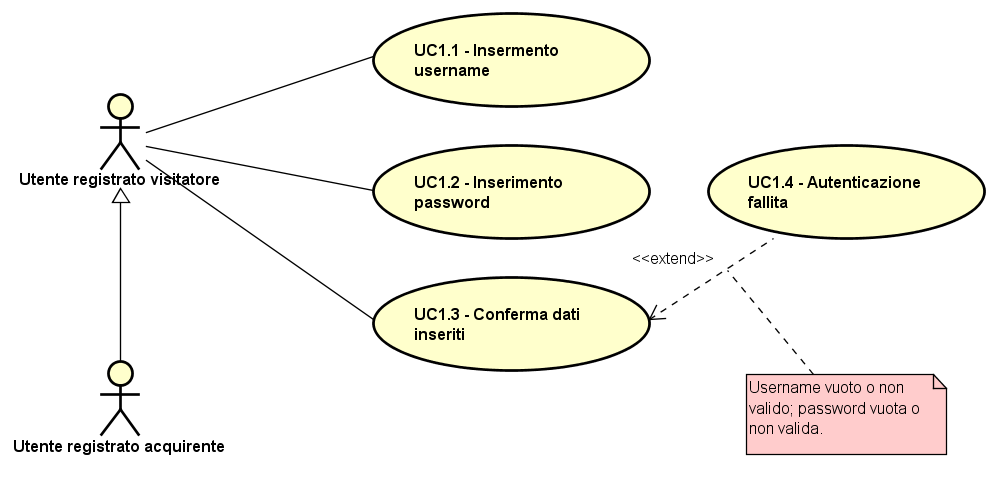
\includegraphics[scale=0.55]{usecase/uc1}
		\caption{UC1: Autenticazione}
	\end{center}
\end{figure}
\FloatBarrier

\subsubsection{Caso d'uso UC2: Interazione con l'ambiente virtuale}

\begin{itemize}
	\item \textbf{Attori:} utente registrato visitatore, utente registrato acquirente;
	\item \textbf{Descrizione:} l'utente, dopo l'autenticazione e collegato il telefono al visore, si ritrova ad osservare un ambiente virtuale con il quale può interagire;
	\item \textbf{Precondizione:} l'utente ha effettuato con successo l'autenticazione;
	\item \textbf{Postcondizione:} l'utente interagisce con gli oggetti presenti nell'ambiente virtuale e se è acquirente può comprare gli oggetti presenti nel carrello;
	\item \textbf{Scenario principale:}
	\begin{enumerate}
		\item L'utente può interagire con un oggetto, segnalato da un apposito simbolo, presente nell'ambiente virtuale (UC2.1);
		\item L'utente può interagire con il carrello presente nell'ambiente e segnalato da un'apposita scritta (UC2.2);
		\item L'utente può uscire dall'applicazione effettuando così il logout (UC2.3).
	\end{enumerate}
\end{itemize}

\label{UC2}
\begin{figure}[ht]
	\begin{center}
		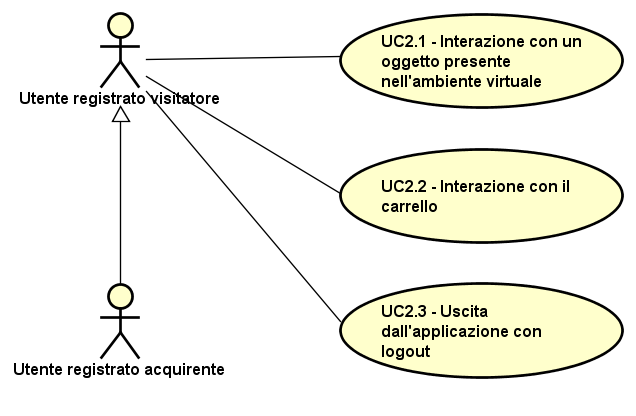
\includegraphics[scale=0.7]{usecase/uc2}
		\caption{UC2: Interazione con l'ambiente virtuale}
	\end{center}
\end{figure}
\FloatBarrier

\subsubsection{Caso d'uso UC2.1: Interazione con un oggetto}

\begin{itemize}
	\item \textbf{Attori:} utente registrato visitatore, utente registrato acquirente;
	\item \textbf{Descrizione:} l'utente interagisce con un oggetto presente nell'ambiente tramite l'interfaccia fisica del visore, attivando il pannello informativo. All'interno di questo sono riportate tutte le informazioni del prodotto e le sue foto. Dal pannello è possibile aggiungere l'oggetto al carrello;
	\item \textbf{Precondizione:} l'utente ha effettuato con successo l'autenticazione;
	\item \textbf{Postcondizione:} l'utente interagisce con l'oggetto attivando il pannello informativo.
	\item \textbf{Scenario principale:}
	\begin{enumerate}
		\item Visualizzazione informazioni dell'oggetto sul pannello informativo (UC2.1.1);
		\item Scorrimento foto dell'oggetto sul pannello informativo (UC2.1.2);
		\item Aggiunta oggetto al carrello selezionando l'apposito pulsante (UC2.1.3).
	\end{enumerate}
\end{itemize}

\label{UC2.1}
\begin{figure}[ht]
	\begin{center}
		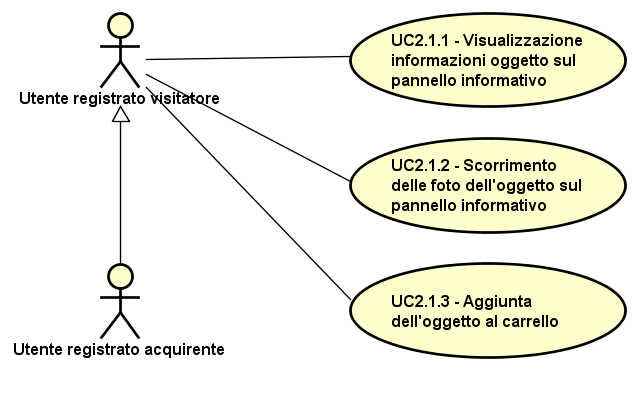
\includegraphics[scale=0.7]{usecase/uc2_1}
		\caption{UC2.1: Interazione con un oggetto}
	\end{center}
\end{figure}
\FloatBarrier

\subsubsection{Caso d'uso UC2.2: Interazione con il carrello}

\begin{itemize}
	\item \textbf{Attori:} utente registrato visitatore, utente registrato acquirente;
	\item \textbf{Descrizione:} entrambe le tipologie possono interagire con il carrello segnalato nell'ambiente da un'apposita scritta. All'interno di esso sono visibili gli oggetti precedentemente inseriti. E' possibile, attraverso l'interfaccia fisica del visore, eliminarli uno ad uno o svuotare completamente il carrello. Se l'utente registrato è acquirente allora può procedere al pagamento;
	\item \textbf{Precondizione:} l'utente ha effettuato l'autenticazione;
	\item \textbf{Postcondizione:} l'utente visualizza i prodotti presenti nel carrello, potendoli acquistare se è acquirente;
	\item \textbf{Scenario principale:}
	\begin{enumerate}
		\item L'utente visualizza il pannello tridimensionale che rappresenta il carrello dove sono elencati i prodotti aggiunti precedentemente (UC2.2.1);
		\item L'utente può eliminare singolarmente un oggetto dal carrello (UC2.2.2);
		\item L'utente può svuotare completamente il carrello (UC2.2.3);
		\item Se l'utente è acquirente allora può procedere con l'acquisto dei prodotti (UC2.2.4);
	\end{enumerate}
\end{itemize}

\label{UC2.2}
\begin{figure}[ht]
	\begin{center}
		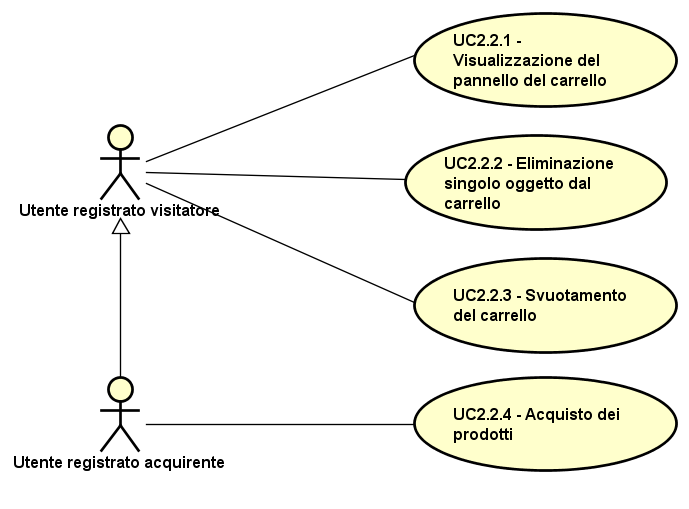
\includegraphics[scale=0.7]{usecase/uc2_2}
		\caption{UC2.2: Interazione con il carrello}
	\end{center}
\end{figure}
\FloatBarrier

\subsection{Requisiti}

Vengono di seguito elencati tutti i requisiti funzionali che l'applicazione deve soddisfare in base ai casi d'uso trovati. Un requisito funzionale rappresenta una \textit{feature} che l'applicazione deve mettere a disposizione all'utente per garantirgli un'esperienza completa. \\
Ogni requisito funzionale è rappresentato da un codice identificativo RFx e da una descrizione che ne illustra lo scopo.

\begin{table}
	\centering
	\label{my-label}
	\begin{tabular}{| l | p{10cm} |}
		\hline
		\textbf{Requisito} & \textbf{Descrizione} \\ \hline
		RF1 & L'applicazione deve permettere all'utente di potersi autenticare utilizzando \textit{username} e \textit{password} specificati in fase di registrazione. \\ \hline
		RF1.1 & L'applicazione deve permettere all'utente di inserire l'\textit{username}. \\ \hline
		RF1.2 & L'applicazione deve permettere all'utente di inserire la \textit{password}. \\ \hline
		RF1.3 & L'applicazione deve permettere all'utente di confermare i dati di autenticazione ed effettuare così il login. \\ \hline
		RF2 & L'applicazione deve permettere all'utente di visualizzare l'ambiente virtuale una volta indossato il visore e di interagire con esso. \\ \hline
		RF2.1 & L'applicazione deve permettere all'utente di interagire con un oggetto presente nella scena attraverso l'interfaccia fisica presente nel visore. \\ \hline
		RF2.1.1 & L'applicazione deve visualizzare le informazioni relative all'oggetto selezionato all'interno di un panello informativo posto davanti all'utente. \\ \hline
		RF2.1.2 & L'applicazione deve permettere la visualizzazione e lo scorrimento delle foto dell'oggetto selezionato all'interno del pannello informativo. \\ \hline
		RF2.1.3 & L'applicazione deve permettere l'aggiunta al carrello dell'oggetto selezionato. \\ \hline
		RF2.2 & L'applicazione deve permettere l'interazione col carrello segnalato da un'apposita scritta all'interno dell'ambiente virtuale. \\ \hline
		RF2.2.1 & L'applicazione deve visualizzare tutti gli oggetti presenti nel carrello precedentemente aggiunti. \\ \hline
		RF2.2.2 & L'applicazione deve permettere all'utente di eliminare un singolo oggetto dal carrello. \\ \hline
		RF2.2.3 & L'applicazione deve permettere di svuotare completamente il carrello. \\ \hline
		RF2.2.4 & L'applicazione deve permettere l'acquisto dei prodotti se l'utente è registrato acquirente. \\ 
		\hline
	\end{tabular}
	\caption{Tabella dei requisiti funzionali che l'applicazione deve soddisfare}
\end{table}
\FloatBarrier

\section{Progettazione}

Questa sezione descrive le più importanti e peculiari fasi di progettazione dell'applicazione. Molte delle decisioni prese sono state discusse da me assieme al \textit{team} di The White Dog s.r.l., cercando il più possibile di accontentare gli \textit{stakeholder}\hyperlink{sh}{\ped{G}}, ovvero il signor Stefano Mocellini, fondatore dell'azienda, attraverso l'ancora giovane e incompleta tecnologia \textit{VR}\ped{\hyperlink{vr}{G}}.

\subsection{Portabilità dell'applicazione}

Una delle sfide più impegnative di questo progetto era riuscire a sviluppare l'applicazione per entrambi i dispositivi: \textit{Samsung Gear VR} e \textit{Google Cardboard}. Prima di conoscere a basso livello tali tecnologie, avevamo progettato l'implementazione di un'interfaccia che riconoscesse la tecnologia in uso e che ne richiamasse così i metodi specifici. Purtroppo, dopo aver sperimentato gli \textit{SDK}\ped{\hyperlink{sdk}{G}} forniti da entrambe le piattaforme e seguito i due principali tutorial\footnote[1]{\textit{Samsung Gear VR:} \url{http://www.samsung.com/us/samsungdeveloperconnection/developer-resources/gear-vr.html} \\ \textit{Google Cardboard:} \url{https://developers.google.com/vr/unity/}}, mi sono reso conto che una totale portabilità non era possibile a causa delle forti differenze tra le due piattaforme. \\ \\
La prima differenza, e la più importante, è la \textbf{MainCamera} o Camera Principale. In un progetto \textit{Unity}, ogni scena possiede una o più camere che rappresentano il punto di vista dell'utente. Una camera normale non permette l'esperienza \textit{VR}\ped{\hyperlink{vr}{G}} poiché non è collegata ai sensori di movimento e rotazione del dispositivo. All'interno dei pacchetti \textit{Unity} offerti agli sviluppatori dalle due case, sono presenti le rispettive camere \textit{VR}\ped{\hyperlink{vr}{G}} che, tramite script ad esse agganciati, permettono l'esperienza \textit{VR}\ped{\hyperlink{vr}{G}} una volta posizionate a piacimento all'interno della scena. Tali script si collegano direttamente ai sensori del dispositivo che è diverso per le due piattaforme. Il visore \textit{Samsung Gear VR} possiede al suo interno tutti i sensori di movimento e rotazione necessari e lo script, agganciato alla \textit{MainCamera}, legge i dati derivanti da essi. Invece, i dispositivi \textit{Google Cardboard} non possiedono alcun sensore e la \textit{MainCamera} legge i dati di rotazione e movimento dai sensori all'interno dello \textit{smartphone}. Questa profonda differenza hardware causa una forte differenza tra i due script della \textit{MainCamera}, obbligando ad inserire una camera specifica per ogni piattaforma all'interno della stessa scena.

\label{MainCamera}
\begin{figure}[ht]
	\begin{center}
		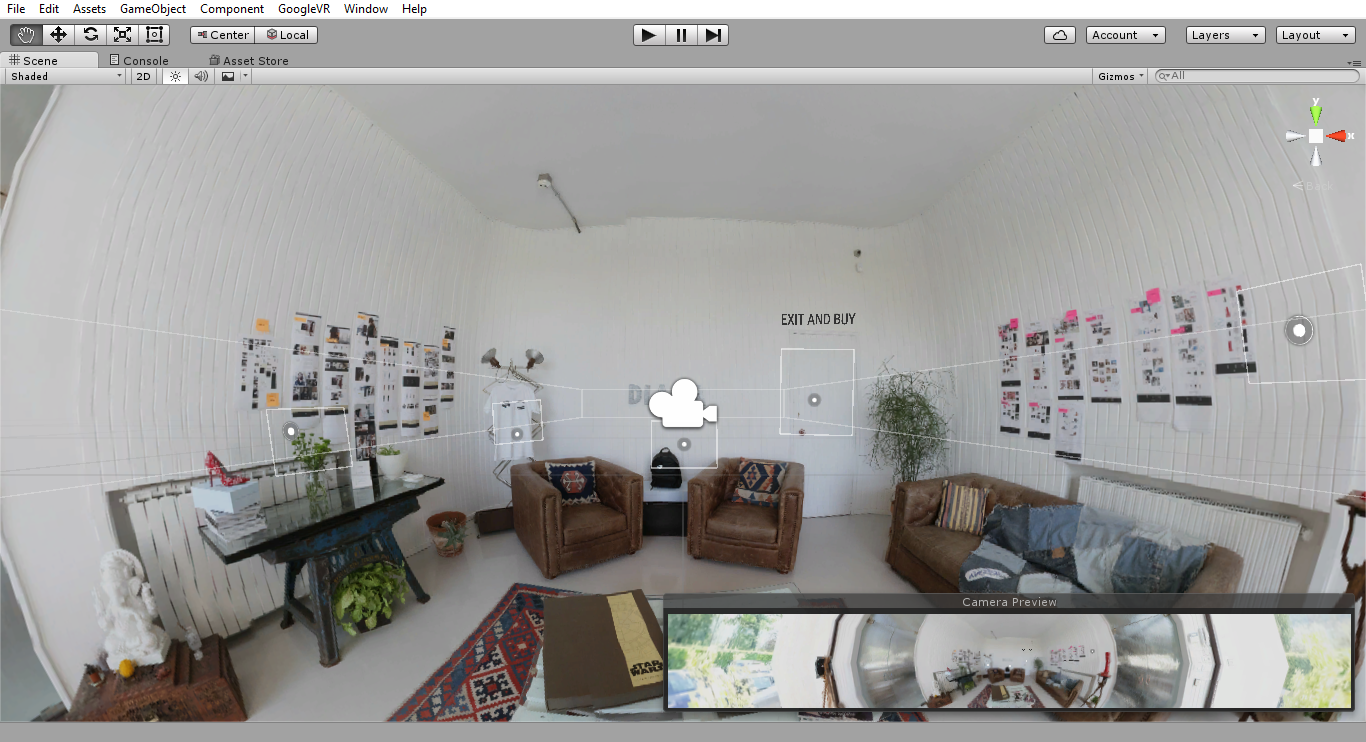
\includegraphics[scale=0.35]{maincamera}
		\caption{Camera VR posizionata all'interno dell'ambiente tridimensionale creato in Unity}
	\end{center}
\end{figure}
\FloatBarrier

La seconda importante differenza è l'implementazione degli \textbf{oggetti interattivi} all'interno della scena \textit{Unity}. Di base, sia per \textit{Samsung Gear VR} sia per \textit{Google Cardboard}, un oggetto per essere interattivo necessità di due caratteristiche:

\begin{itemize}
	\item \textbf{Mesh Collider:} è necessario aggiungere tale proprietà all'oggetto che si vuole rendere interattivo. Tale proprietà rende un oggetto "tangibile", ovvero può essere colliso da un altro oggetto presente nella scena. Questo permette alla \textit{Camera VR} di interagire con l'oggetto inviando un "raggio virtuale" verso quest'ultimo che, scontrandovisi, potrà attivare gli eventi che si desidera;
	\item \textbf{InteractiveScriptVR:} script, da agganciare all'oggetto, che cattura l'evento di selezione attraverso i metodi esposti dall'\textit{api} della particolare piattaforma. All'interno di questi metodi si può implementare il vero comportamento dell'oggetto interattivo.  
\end{itemize}

L'\texttt{InteractiveScriptVR} differisce profondamente da una piattaforma all'altra. \\
Per quanto riguarda \textit{Google Cardboard}, lo script implementa la classe \texttt{IGvrGazeResponder}, la quale espone i metodi per la cattura della selezione tramite lo spostamento del magnete posto lateralmente nel visore. \\
Per quanto riguarda \textit{Samsung Gear VR} invece, l'\texttt{InteractiveScriptVR} non implementa alcuna interfaccia ma necessita l'utilizzo del namespace \texttt{VRStandardAsset.Utils} per richiamare i metodi esposti dallo script \texttt{VRInteractiveItem}, script che va agganciato all'oggetto assieme all'\texttt{InteractiveScriptVR}. \\
Questa differenza di implementazione degli oggetti interattivi rende davvero difficoltosa la loro portabilità da una piattaforma all'altra. Dunque, dopo una lunga discussione avvenuta nell'ufficio R\&D, abbiamo deciso di abbandonare la totale portabilità dell'applicazione, raggiungendo però un compromesso: la separazione della cattura dell'evento di selezione dall'effettivo comportamento dell'oggetto, implementandoli in due script differenti. Il primo, che cambia da piattaforma a piattaforma, richiama il secondo dopo aver catturato l'evento di selezione, il quale rappresenta il vero comportamento dell'oggetto ed è indipendente dalla piattaforma in uso. In questo modo è stato possibile creare dei \textit{prefabs} (oggetti portabili all'interno dell'ambiente \textit{Unity} contenenti le informazioni di forma, colore, script agganciati eccetera) che contenessero solo le informazioni del comportamento dell'oggetto dopo la cattura della selezione.    

\subsection{Usabilità dell'applicazione}

La fase di acquisto inizialmente prevista comprendeva l'immissione dei propri dati di pagamento all'interno dell'ambiente \textit{VR}\ped{\hyperlink{vr}{G}} tramite una tastiera tridimensionale posta davanti all'utente, dove ogni tasto era selezionabile attraverso l'interfaccia fisica del visore. Dopo la sperimentazione di tale tastiera, abbiamo constatato la sua scarsa usabilità, causando un processo d'acquisto lungo e tedioso. Abbiamo dunque optato per una soluzione più semplice: l'utente prima di entrare nella scena \textit{VR}\ped{\hyperlink{vr}{G}} viene invitato a immettere i propri dati di login attraverso la normale tastiera del telefono, così da accedere al proprio account personale. Tale account deve essere precedentemente creato nel sito/e-commerce dedicato, dove possono essere immessi anche i dati di pagamento. L'implementazione di tale sito esce dagli obbiettivi di questo progetto, dunque non mi sono occupato dello sviluppo di quest'ultimo. Una volta autenticato, lo \textit{smartphone} passa in modalità \textit{VR}\ped{\hyperlink{vr}{G}}, invitando l'utente ad indossare il visore. All'interno dell'ambiente, all'utente non viene più richiesto di immettere dati, così da poter sperimentare in tutta serenità l'esperienza \textit{VR}\ped{\hyperlink{vr}{G}}. \\
Questa soluzione però ha mostrato al \textit{team} la profonda differenza tra le piattaforme \textit{Samsung Gear VR} e \textit{Google Cardboard}. Ogni applicazione \textit{Samsung Gear VR}, una volta avviata, richiede all'utente di inserire lo \textit{smartphone} all'interno del visore prima di poter effettivamente essere utilizzata. Questo obbliga lo sviluppatore a prevedere tutte scene di tipo \textit{VR}\ped{\hyperlink{vr}{G}} durante lo sviluppo dell'applicazione, contrariamente a \textit{Google Cardboard} che permette la coesistenza di tutte le tipologie scenografiche: 2D, 3D e \textit{VR}\ped{\hyperlink{vr}{G}}. Dunque, non è stato possibile inserire una scena 2D iniziale di login per la piattaforma Samsung e, a causa dei tempi ridotti di stage, non è stato possibile sviluppare una soluzione a tale problema.

\label{Login}
\begin{figure}[ht]
	\begin{center}
		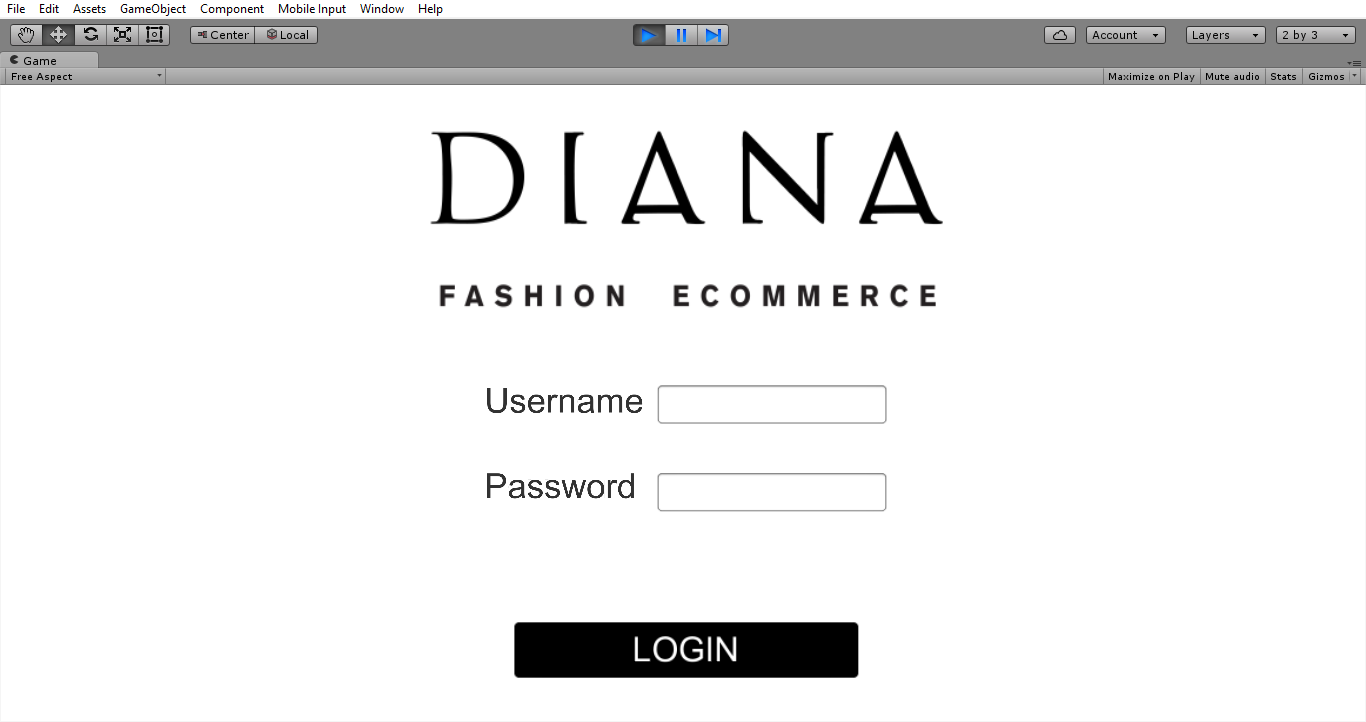
\includegraphics[scale=0.35]{login}
		\caption{Schermata 2D di login}
	\end{center}
\end{figure}
\FloatBarrier

\subsection{Costruzione della scena 3D}

Dopo un'attenta fase di ricerca iniziale sulla tecnologia \textit{Unity} e \textit{VR}\ped{\hyperlink{vr}{G}}, ho potuto constatare che vi sono due modi principali per costruire una scena 3D:

\begin{itemize}
	\item \textbf{Tramite modellazione 3D dell'intero ambiente virtuale};
	\item \textbf{Tramite l'applicazione di una foto a 360 gradi di una stanza ad una sfera o cubo inversi}.
\end{itemize}

La prima soluzione permette una vera esperienza 3D, dando la possibilità all'utente di spostarsi nelle tre dimensioni, prevedendo l'utilizzo di un gamepad. Ogni oggetto è ben definito in un punto dello spazio tridimensionale e osservabile da tutte le angolazioni. Purtroppo però per costruire un ambiente 3D di qualità accettabile sono necessarie profonde conoscenze di modellazione, conoscenze che fuoriescono dall'obbiettivo di questo stage. \\
La seconda soluzione non permette una totale esperienza 3D, poiché applica una foto 2D a 360 gradi ad una sfera o un cubo inversi creati in \textit{Unity}. L'effetto così creato simula la tridimensionalità, non permettendo all'utente lo spostamento tra gli oggetti ma solo una visione stereoscopica della stanza. Il livello qualitativo raggiunto però è ottimo, se la foto viene realizzata con le giuste apparecchiature. Abbiamo deciso dunque di utilizzare la seconda metodologia per la creazione dell'ambiente. \\
Abbiamo così realizzato la foto a 360 gradi utilizzando una macchinetta fotografica di alta qualità presente nell'azienda seguendo la guida presente nel sito: lightspacewater\footnote[2]{\url{http://www.lightspacewater.net/Tutorials/PhotoPano2/paper/}}. \\
Posizionata la macchinetta fotografica sul cavalletto al centro di una stanza, appositamente arredata allo scopo, dell'azienda Diana Corp., abbiamo effettuato 3 foto, una sovraesposta, una sottoesposta e una ad esposizione normale, ogni 45 gradi orizzontalmente. Abbiamo poi ripetuto l'operazione inclinando la macchinetta 45 gradi verso il basso ed infine 45 gradi verso l'alto. \\ 
Le foto così ottenute, ci hanno permesso di creare la foto a 360 gradi tramite il software Autopano\footnote[3]{\url{http://www.kolor.com/autopano/}}, che l'ha creata automaticamente a meno di qualche punto di agganciamento inserito manualmente. Infine abbiamo applicato la foto come texture di una sfera inversa creata tramite l'editor di \textit{Unity}.

\label{Sfera}
\begin{figure}[ht]
	\begin{center}
		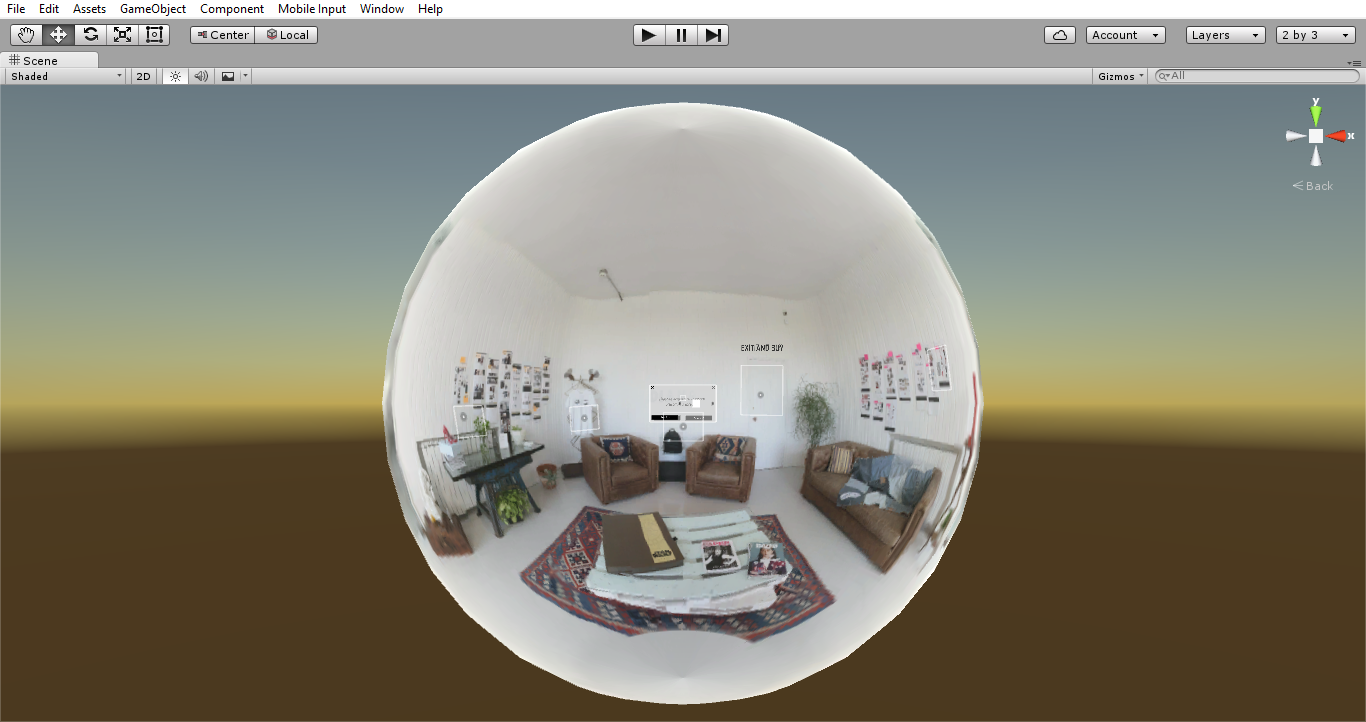
\includegraphics[scale=0.35]{sfera}
		\caption{Sfera inversa a cui è stata applicata la foto 360 della stanza come texture}
	\end{center}
\end{figure}
\FloatBarrier  

\subsection{Interazione con gli oggetti all'interno della scena} 

All'interno della scena creata tramite la foto a 360 gradi, gli oggetti presenti nella stanza non sono veri oggetti tridimensionali modellati in \textit{Unity}. A quest'ultimi, come descritto nella sezione 3.5.1, è possibile applicare la proprietà \textit{Mesh Collider}, per renderli tangibili, e lo script che cattura l'evento di selezione. Purtroppo nella soluzione da noi adottata gli oggetti fanno parte della foto che crea lo sfondo, perciò non è possibile applicargli queste due proprietà. \\
Abbiamo così deciso di porre davanti ad ogni oggetto un pannello tridimensionale creato tramite l'editor di \textit{Unity} e ad esso agganciargli le caratteristiche citate. In più al pannello viene disabilitata la proprietà \textit{Mesh Renderer}, proprietà che lo rende visibile. \\ 
In questo modo viene simulata l'interattività dell'oggetto che, alla selezione tramite l'interfaccia fisica del visore, attiva il pannello informativo relativo all'oggetto selezionato.

\label{Oggetto Interattivo}
\begin{figure}[ht]
	\begin{center}
		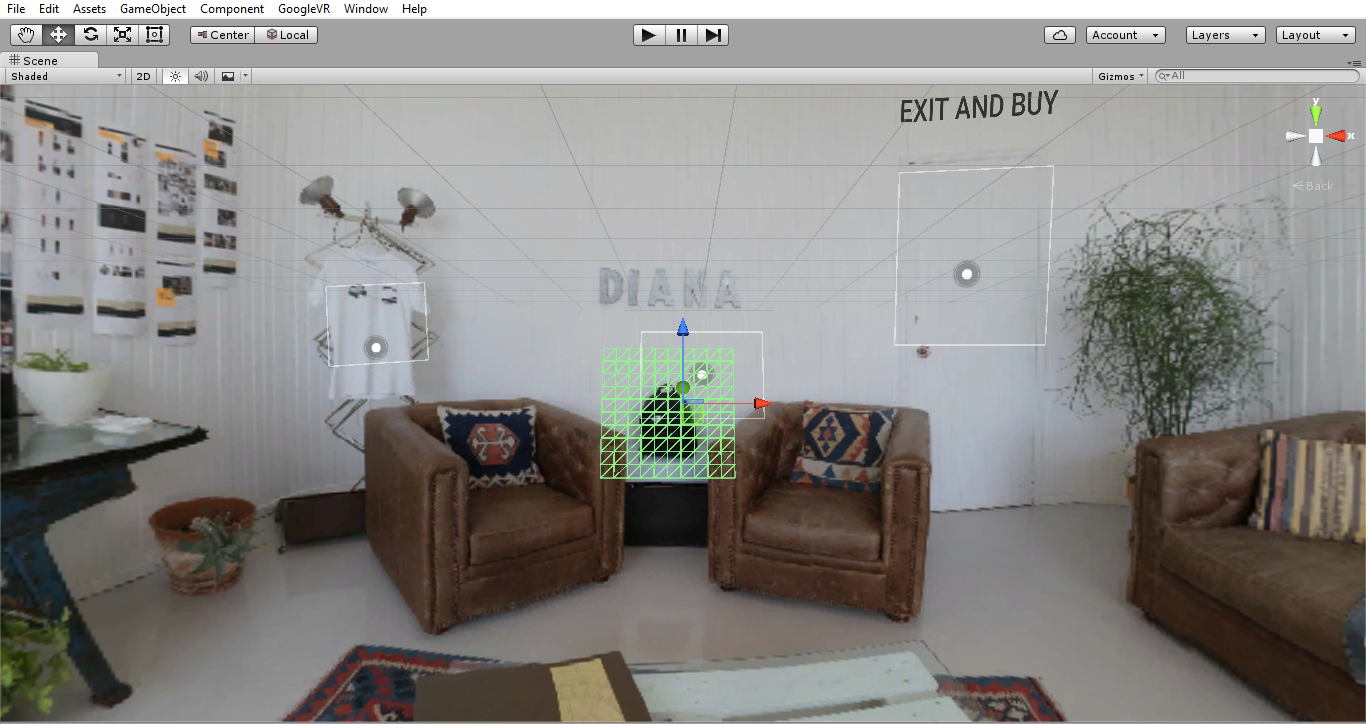
\includegraphics[scale=0.35]{pannello}
		\caption{Pannello tridimensionale posto davanti ad un oggetto presente nella stanza per renderlo interattivo}
	\end{center}
\end{figure}
\FloatBarrier  

\subsection{Progettazione e integrazione con AWS API Gateway}

Uno degli obiettivi dello stage era sperimentare la comunicazione tra l'applicazione creata con \textit{Unity} e sistemi esterni tramite protocollo HTTP, come ad esempio un \textit{e-commerce}. Per testare tali funzionalità in sicurezza, senza dover creare o modificare gli \textit{e-commerce} aziendali, il tutor mi ha suggerito di utilizzare il servizio \textit{API Gateway} di \textit{Amazon Web Service}. Amazon API Gateway è un servizio completamente gestito che semplifica agli sviluppatori la creazione, la pubblicazione, la manutenzione, il monitoraggio e la protezione delle API su qualsiasi scala. Essa agisce come porta d'entrata attraverso la quale le applicazioni possono accedere a dati, logica di business o funzionalità dei servizi di back-end. Gestisce tutte le attività di accettazione ed elaborazione relative alle chiamate API simultanee, inclusi gestione del traffico, controllo di accessi e autorizzazioni, monitoraggio e gestione delle versioni delle API. Infine permette la creazione di \textit{API Mock}, ovvero API che non si agganciano ad alcun back-end ma che rispondono messaggi prefissati ad ogni chiamata HTTP. Quest'ultima funzionalità ci ha spinto ad utilizzare questo servizio, dato che lo sviluppo di un vero back-end non rientrava all'interno degli obiettivi di stage. \\
Ho creato dunque tre risorse e al loro interno le relative chiamate HTTP:
\begin{itemize}
	\item \textbf{/login}: risorsa riguardante le operazioni di autenticazione. Contiene la chiamata:
	\begin{itemize}
		\item POST: riceve un file JSON contenente l'username e la password immesse dall'utente e restituisce un \textit{token} di autenticazione.
	\end{itemize}
	\item \textbf{/products}: risorsa riguardante le operazione sui prodotti. Contiene la chiamata:
	\begin{itemize}
		\item GET: ritorna un file JSON contenente le informazioni riguardanti tutti i prodotti all'interno della scena come nome, descrizione e foto.
	\end{itemize}
	\item \textbf{/products/{id}}: risorsa riguardante le operazioni su un singolo prodotto. Contiene la chiamata:
	\begin{itemize}
		\item GET: ritorna un file JSON contenente le informazioni su un singolo prodotto in base all'id passato. 
	\end{itemize}
	\item \textbf{/cart}: risorsa riguardante le operazioni sul carrello. Contiene le chiamate:
	\begin{itemize}
		\item POST: riceve un file JSON contenente i prodotti presenti all'interno del carrello.
	\end{itemize} 
\end{itemize}

\label{AWS API Gateway}
\begin{figure}[ht]
	\begin{center}
		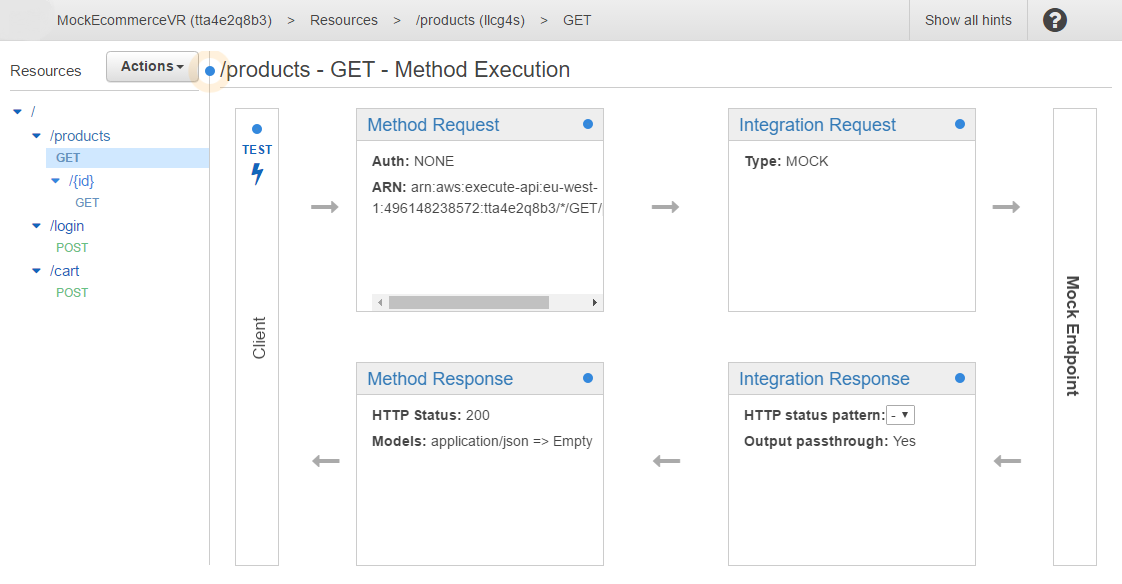
\includegraphics[scale=0.45]{aws}
		\caption{Flusso della chiamata GET all'interno della risorsa \textit{/products} in AWS API Gateway}
	\end{center}
\end{figure}
\FloatBarrier

Per quanto riguarda \textit{Unity}, invece, ho sfruttato la classe \texttt{WWW} che consente di effettuare chiamate GET per recuperare dati JSON o foto:

\begin{lstlisting}[firstnumber=1]
string url = "https://tta4e2q8b3.execute-api.eu-west-1.amazonaws.com/prod/products";

WWW www = new WWW(url);
\end{lstlisting}

e chiamate POST, potendo inviare \textit{headers} e corpo:

\begin{lstlisting}[firstnumber=1]
string url = "https://tta4e2q8b3.execute-api.eu-west-1.amazonaws.com/prod/login";

string JSON = "{\"username\" : " + "\"" + Username + "\", " + "\"password\" : " + "\"" + Password + "\"}";
	
byte[] body = System.Text.Encoding.UTF8.GetBytes(JSON);    
	
Dictionary<string, string> headers = new Dictionary<string, string>();
	
headers.Add( "Content-Type", "application/json" );
	
headers.Add( "X-HTTP-Method-Override", "POST" );
	
WWW www = new WWW(url, body, headers);
\end{lstlisting}

\section{Sviluppo}

In questa sezione andrò a descrivere in dettaglio lo sviluppo delle più significative e peculiari funzionalità dell'applicazione.

\subsection{Spostamento degli oggetti all'interno dell'ambiente tridimensionale}

\subsection{Creazione a runtime di oggetti interattivi}

In questa sottosezione tratterò della creazione a runtime di oggetti interattivi in Unity.

\subsection{Dati persistenti attraverso le scene}

In questa sezione spiegherò come si costruiscono oggetti persistenti che vivono attraverso le scene.

\subsection{Creazione e parsing di oggetti JSON in Unity}

In questa sottosezione parlerò di come si creino e si manipolino oggetti JSON in Unity.            
\newpage
%**************************************************************
% CAPITOLO 4
%**************************************************************
\chapter{Analisi retrospettiva}
\label{cap:analisiretrospettiva}

\section{Bilancio dei risultati rispetto agli obiettivi prefissati}

Come affermato dal tutor aziendale, gli obbiettivi che l'azienda aveva fissato nel piano di lavoro rappresentavano le aspettative che gli \textit{stakeholder}\hyperlink{sh}{\ped{G}} avevano sulla tecnologia \textit{VR}\ped{\hyperlink{vr}{G}}, senza però essere avvalorate da alcuna conoscenza specifica. Nemmeno il \textit{team} R\&D, reparto di ricerca e sviluppo, era riuscito ad approfondirne lo studio, a causa di impegni aziendali più prioritari. Dunque, non erano certi che tali obbiettivi potessero essere soddisfatti, lasciandomi così completa libertà sia per quanto riguarda le tecnologie da adottare sia per quanto riguarda le tempistiche. Questa libertà mi ha permesso di raggiungere molti degli obiettivi primari, che sono andati definendosi maggiormente con l'aumento della mia personale conoscenza sulle tecnologie:
\begin{itemize}
	\item \textbf{Prototipo scena 3D:} come discusso nel paragrafo 3.2.3 abbiamo deciso di costruire la scena attraverso una foto a 360 gradi di una stanza applicata ad una sfera inversa invece che modellare l'intera scena con oggetti 3D;
	\item \textbf{Progettazione e sviluppo di oggetti e comportamento di essi nello spazio 3D:} come discusso nei paragrafi 3.2.3 e 3.2.4 gli oggetti non sono stati modellati attraverso l'editor grafico di \textit{Unity}, ma ho posto dei pannelli interattivi invisibili davanti agli oggetti che compongono la scena a 360 gradi;
	\item \textbf{Progettazione e sviluppo integrazione tra sistema di VE e e-commerce:} come discusso nel paragrafo 3.2.5 l'applicazione non è stata integrata con un vero \textit{e-commerce} ma con un API creata tramite \textit{Amazon Web Service};
	\item \textbf{Approfondimento di user interactions (Leap Motion, eccetera):} presa la decisione della strada \textit{mobile}, le uniche \textit{user interaction} possibili erano tramite i due dispositivi \textit{VR}\ped{\hyperlink{vr}{G}} presenti in azienda: \textit{Samsung Gear VR} e \textit{Google Cardboard};
	\item \textbf{Studio e prototipazione del possibile processo di acquisto all’interno di un VE (registrazione, checkout, pagamenti eccetera):} come discusso nel paragrafo 3.2.2 è stato scelto di permettere all'utente una registrazione ad un normale \textit{e-commerce}, con la possibilità di immettere i dati di pagamento, prima dell'utilizzo dell'applicazione.
\end{itemize} 

\begin{table}
	\centering
	\label{tabella-obbiettivi}
	\begin{tabular}{| p{6cm} | p{6cm} |}
		\hline
		\textbf{Obiettivo} & \textbf{Realizzazione} \\ \hline
		 \textbf{Minimo:} Studio delle tecnologie disponibili in ambito \textit{VR}\ped{\hyperlink{vr}{G}} e stesura di un documento riassuntivo che offra un \textit{overview} dello stato attuale della realtà aumentata. &  \textbf{Obbiettivo realizzato:} è stato redatto un documento che riporta tutte le tecnologie VR presenti nel mercato e i rispettivi stack tecnologici.\\ \hline
		 \textbf{Minimo:} Progettazione e sviluppo di un ambiente virtuale con: una scena e oggetti definiti, un comportamento associato agli oggetti, un prototipo di \textit{user interaction}. & \textbf{Obbiettivo realizzato:} come esposto nei paragrafi 3.2.3, 3.2.4, 3.3.2 e 3.3.4 gli obbiettivi di realizzazione della scena, degli oggetti e del loro comportamento e della \textit{user interaction} sono stati portati a termine. \\ \hline
		 \textbf{Minimo:} Scambio di informazioni di base tra l'applicazione e un sistema di \textit{e-commerce}. & \textbf{Obiettivo parzialmente realizzato:} l'integrazione con un \textit{e-commerce} è stata in parte realizzata come descritto nella sezione 3.2.5.\\ \hline
		 \textbf{Massimo:} Studio e prototipazione di diversi modelli di \textit{user interaction} con l'ambiente e con gli oggetti finalizzati alla presentazione di un bene vendibile. & \textbf{Obbiettivo parzialmente realizzato:} presa la decisione di intraprendere la strada \textit{mobile}, i possibili modelli di \textit{user interaction} erano due: \textit{Samsung Gear VR} e \textit{Google Cardboard}. Come esposto nel paragrafo 3.2.1, la portabilità dell'applicazione nei due ambienti di studio non è stata completamente implementabile.\\ \hline
		 \textbf{Massimo:} Studio e implementazione di possibili nuovi processi di acquisto in ambito \textit{VR}\ped{\hyperlink{vr}{G}}. & \textbf{Obbiettivo parzialmente realizzato:} come esposto nella sezione 3.2.2 sono stati studiati diversi processi d'acquisto in ambito \textit{VR}\ped{\hyperlink{vr}{G}} ed uno di questi è stato in parte realizzato.\\ \hline
	\end{tabular}
	\caption{Tabella degli obbiettivi minimi e massimi aziendali discussi nella sezione 2.2.2, con affianco il loro grado di realizzazione}
\end{table}
\FloatBarrier

Nonostante non sia riuscito a portare a termine alcuni obbiettivi, mi ritengo pienamente soddisfatto per i molti che invece sono riuscito realizzare. La tecnologia che ho dovuto utilizzare per la realizzazione di questo progetto, era a me completamente sconosciuta e molti degli obbiettivi non realizzati, come discusso nel capitolo 3, sono risultati essere impossibili da portare a termine a causa dell'immaturità della tecnologia \textit{VR}\ped{\hyperlink{vr}{G}}. \\ 
Il più importante obbiettivo di questo stage era sperimentare le potenzialità e i limiti della realtà virtuale applicata all'ambito \textit{e-commerce} e tale obbiettivo è stato completamente portato a termine, come confermatomi dal tutor aziendale.

\section{Bilancio formativo}

Il bagaglio culturale che questa attività di stage mi ha permesso di creare è formato sostanzialmente da due parti. \\
La prima è costituita dalle \textbf{conoscenze tecnologiche} apprese, le quali non fanno parte del normale percorso universitario. La costruzione di ambienti e oggetti tridimensionali e lo sviluppo del loro comportamento, sono campi dell'informatica davvero interessanti da studiare e sperimentare, tanto che vi sono scuole che offrono interi master sull'argomento. Ad oggi, la computer grafica non è più circoscritta solo all'ambito videoludico ma viene utilizzata in maniera massiccia in molti altri campi come quello cinematografico e pubblicitario. Essa, dunque, rappresenta un notevole valore aggiunto per quanto riguarda il curriculum personale. La seconda tecnologia che lo stage mi ha permesso di studiare, e che non rientra nei corsi universitari, è \textit{API Gateway} di \textit{Amazon Web Service}. Amazon si sta affermando come una delle più importanti piattaforme di servizi di \textit{cloud computing}\hyperlink{cc}{\ped{G}} e lo sviluppo di un API tramite questa tecnologia mi ha permesso di comprendere meglio la natura della comunicazione tra i servizi di front-end e back-end. Infine, anche se gli strumenti per lo sviluppo \textit{VR}\ped{\hyperlink{vr}{G}} sono risultati essere in parte incompleti, la realtà virtuale è sicuramente una delle tecnologie emergenti e più influenti dell'ultimo anno. Molte gradi aziende come Sony, Microsoft, Samsung e Google stanno investendo molto in questo settore, destinato a cambiare radicalmente la nostra quotidiana esperienza multimediale e videoludica. Poterne studiare il processo evolutivo e le sue attuali potenzialità è stato per me davvero affascinate e coinvolgente. \\
La seconda parte che va a formare il bagaglio culturale creato con l'attività di stage è sicuramente \textbf{l'esperienza aziendale}, parte che tra le due ritengo la più importante. La collaborazione con i colleghi, il rapporto con il datore di lavoro e gli \textit{stakeholder}\hyperlink{sh}{\ped{G}}, il rispetto degli orari, della sicurezza e della regolamentazione costituiscono un'esperienza fondamentale per uno studente di un indirizzo orientato al mondo del lavoro. Poter usufruire di un servizio universitario che garantisce un'esperienza lavorativa all'interno del percorso di studi permette a tutti gli studenti che entrano per la prima volta nel mondo del lavoro di conoscere già le dinamiche generali aziendali così da poter fin da subito adattarvisi. \\
Ritengo dunque il bilancio formativo davvero positivo e posso affermare che lo stage rappresenta una delle più importanti attività svolte nel mio personale percorso universitario.

\section{Analisi critica del rapporto formativo tra stage e corso di laurea}

Molte sono le conoscenze apprese durante il percorso universitario che mi hanno aiutato nell'attività di stage. In particolare, sono tre i corsi che maggiormente hanno influito sul corretto sviluppo dell'applicazione: Programmazione, Programmazione ad oggetti e Ingegneria del Software. \\
Il corso di \textbf{Programmazione} mi ha aiutato molto nella gestione delle strutture dati di base, nella creazione degli algoritmi e dei cicli iterativi innestati. Gli array dinamici e circolari, supportati da algoritmi efficienti, mi hanno permesso lo sviluppo di molte caratteristiche interessanti come il carrello logico e lo slide di immagini. \\
Il corso di \textbf{Programmazione ad oggetti} mi ha permesso innanzitutto la comprensione dell'architettura degli \textit{SDK}\ped{\hyperlink{sdk}{G}} forniti da Samsung e Google per lo sviluppo \textit{VR}\ped{\hyperlink{vr}{G}}. Molte classi offerte implementano interfacce o derivano altre classi, ed essere riuscito a comprenderne fin da subito il flusso gerarchico mi ha aiutato a rispettare gli obbiettivi settimanali. In più, ho potuto applicare tali concetti sviluppando io stesso moltissime classi ed una loro gerarchia. Tutti gli script che definiscono il comportamento degli oggetti sono in realtà realizzati attraverso classi che si occupano della gestione logica dell'oggetto. Anche la portabilità dell'applicazione attraverso le due piattaforme è stata possibile solo grazie a queste conoscenze, poiché mi ha permesso di creare classi indipendenti dalla particolare tecnologia \textit{VR}\ped{\hyperlink{vr}{G}}, come ad esempio la classe che effettua il parsing degli oggetti JSON o la classe che si occupa della gestione dei dati persistenti attraverso le scene. \\
Infine, il corso di \textbf{Ingegneria del Software} non mi ha aiutato in una tecnologia in particolare, ma nella visione d'insieme e nel rapporto con il \textit{team} di sviluppo. Nonostante il progetto di Ingegneria del Software sia stato su tecnologie differenti, la metodologia di lavoro appresa grazie ad esso mi ha aiutato molto nella progettazione, nella scelta del ciclo di vita, nel rapporto con i colleghi, nella stesura della documentazione e soprattutto nelle ricerca delle conoscenze. Ogni corso universitario viene trattato come una scatola chiusa, un'ambiente che sembra non comunicare con gli altri, vivendo solo all'interno di se stesso. Ingegneria del Software ti spinge ad uscire da queste scatole e ricercare i collegamenti fra esse, scoprendo così che non vi sono limiti. \\
Vi è però un'ambito dell'informatica che purtroppo non viene trattato nel percorso di studi e la sua mancanza ha influito negativamente nel mio personale progetto di stage, ovvero la \textbf{computer grafica}. Comprendo la forte difficoltà nel creare un corso di pochi mesi su un argomento così vasto e mutevole. Oltretutto, è una materia davvero settoriale e pochi sono i punti di contatto con le altre materie informatiche. Ma trattarne anche solo i principi di base, costituirebbe un notevole valore aggiunto al corso di studi, se non addirittura all'intera Università. Molti studenti oggi vengono attratti dall'informatica perché appassionati di hardware e del mondo videoludico. Un corso, anche opzionale, che tocchi tali temi permetterebbe allo studente appassionato di proseguire con molto più impegno e dedizione il percorso di studi scelto.  

\section{Valutazioni personali}

Fin dagli albori della contemporanea realtà virtuale, ho sempre pensato che l'utenza non fosse ancora pronta per una tale rivoluzione multimediale. Da subito essa ha ricevuto numerose critiche da chi sostiene che sia un mezzo per il totale distacco dalla realtà. Oltretutto, è lungi da offrire una qualità grafica al pari degli attuali monitor e televisori e, a causa della vertiginosa crescita tecnologica degli ultimi anni, è ormai difficile accogliere una nuova tecnologia che non sia in tutto migliore di quella precedente. Per poter sperimentare la massima esperienza \textit{VR}\ped{\hyperlink{vr}{G}} ad oggi possibile, è necessario un hardware di fascia alta, hardware non accessibile all'utenza media, l'unica in grado di trasformare una nuova tecnologia in uno standard. Inoltre i dispositivi meno costosi sono troppo lontani dall'attuale qualità multimediale e investire in loro con nessuna certezza di miglioramento è davvero pionieristico. Infine, il lavoro degli sviluppatori, che si affacciano per la prima volta alla realtà virtuale, non è decisamente agevolato data l'immaturità degli \textit{SDK}\ped{\hyperlink{sdk}{G}} disponibili e la totale mancanza di uno standard. \\ 
Tutto ciò porterebbe ad una visione negativa della realtà virtuale, se non si riuscisse a vedere le sue reali potenzialità. Poter vivere l'esperienza \textit{VR}\ped{\hyperlink{vr}{G}} mi ha reso consapevole del fascino che essa può offrire e delle emozioni che è in grado di regalare. Cambiare stanza, regione o Paese, immergersi completamente all'interno di un'azione di un film, interagire con l'ambiente circostante per conoscerne in tempo reale le informazioni, da oggi è possibile solamente indossando un visore. \\
La realtà virtuale è sicuramente ancora in fase embrionale, fase che durerà a lungo. Ma sono convinto che essa inesorabilmente entrerà nella nostra quotidianità, cambiando radicalmente il nostro modo di vivere la multimedialità è il nostro rapporto con la realtà. Sta a ognuno di noi trovarne il giusto utilizzo.           
\facciatabianca                   
%**************************************************************
% Materiale finale
%**************************************************************
\backmatter
%\printglossaries
% 
\input{glossario}  
\newpage
%**************************************************************
% Bibliografia
%**************************************************************

\cleardoublepage
\appendix


\chapter{Bibliografia}

\subsubsection{Siti web consultati}

\begin{itemize}
	\item \textbf{Diana Corp.}	\url{http://www.dianacorp.com/}
	\item \textbf{Live Story}	\url{http://www.livestory.nyc/}
	\item \textbf{Manifesto Agile}	\url{http://agilemanifesto.org/}
	\item \textbf{Smasung Gear VR}	\url{http://www.samsung.com/us/samsungdeveloperconnection/developer-resources/gear-vr.html}
	\item \textbf{Google Cardboard}	\url{https://vr.google.com/cardboard/}
	\item \textbf{Amazon Web Services}	\url{https://aws.amazon.com/it/}
	\item \textbf{Unity}	\url{https://unity3d.com/}
	\item \textbf{Ligthspacewater}	\url{http://www.lightspacewater.net/Tutorials/PhotoPano2/paper/}
	\item \textbf{LitJSON}	\url{https://lbv.github.io/litjson/}
	\item \textbf{TSW}	\url{http://www.tsw.it/digital-marketing/}
	\item \textbf{folio3}	\url{http://www.folio3.com/blog/}
\end{itemize}
\end{document}